\documentclass[10pt,landscape]{article}
\usepackage{multicol}
\usepackage{calc}
\usepackage{ifthen}
\usepackage[landscape]{geometry}
\usepackage{amsmath,amsthm,amsfonts,amssymb}
\usepackage{color,graphicx,overpic}
\usepackage{hyperref}

\pdfinfo{
/Title (example.pdf)
/Creator (TeX)
/Producer (pdfTeX 1.40.0)
/Author (Seamus)
/Subject (Example)
/Keywords (pdflatex, latex,pdftex,tex)}

% This sets page margins to .5 inch if using letter paper, and to 1cm
% if using A4 paper. (This probably isn't strictly necessary.)
% If using another size paper, use default 1cm margins.
\ifthenelse{\lengthtest { \paperwidth = 11in}}
{ \geometry{top=.5in,left=.5in,right=.5in,bottom=.5in} }
{\ifthenelse{ \lengthtest{ \paperwidth = 297mm}}
{\geometry{top=1cm,left=1cm,right=1cm,bottom=1cm} }
{\geometry{top=1cm,left=1cm,right=1cm,bottom=1cm} }
}

% Turn off header and footer
\pagestyle{empty}

% Redefine section commands to use less space
\makeatletter
\renewcommand{\section}{\@startsection{section}{1}{0mm}%
{-1ex plus -.5ex minus -.2ex}%
{0.5ex plus .2ex}%x
{\normalfont\large\bfseries}}
\renewcommand{\subsection}{\@startsection{subsection}{2}{0mm}%
{-1explus -.5ex minus -.2ex}%
{0.5ex plus .2ex}%
{\normalfont\normalsize\bfseries}}
\renewcommand{\subsubsection}{\@startsection{subsubsection}{3}{0mm}%
{-1ex plus -.5ex minus -.2ex}%
{1ex plus .2ex}%
{\normalfont\small\bfseries}}
\makeatother

% Define BibTeX command
\def\BibTeX{{\rm B\kern-.05em{\sc i\kern-.025em b}\kern-.08em
T\kern-.1667em\lower.7ex\hbox{E}\kern-.125emX}}

% Don't print section numbers
\setcounter{secnumdepth}{0}


\setlength{\parindent}{0pt}
\setlength{\parskip}{0pt plus 0.5ex}

%My Environments
\newtheorem{example}[section]{Example}
% -----------------------------------------------------------------------

\begin{document}
\raggedright
% \footnotesize
\scriptsize
\begin{multicols}{4}
    
    
    % multicol parameters
    % These lengths are set only within the two main columns
    %\setlength{\columnseprule}{0.25pt}
    \setlength{\premulticols}{1pt}
    \setlength{\postmulticols}{1pt}
    \setlength{\multicolsep}{1pt}
    \setlength{\columnsep}{2pt}
    
    % \begin{center}
        %     \Large{\underline{Title}} \\
    % \end{center}
    \section{Instance Based Learning}

    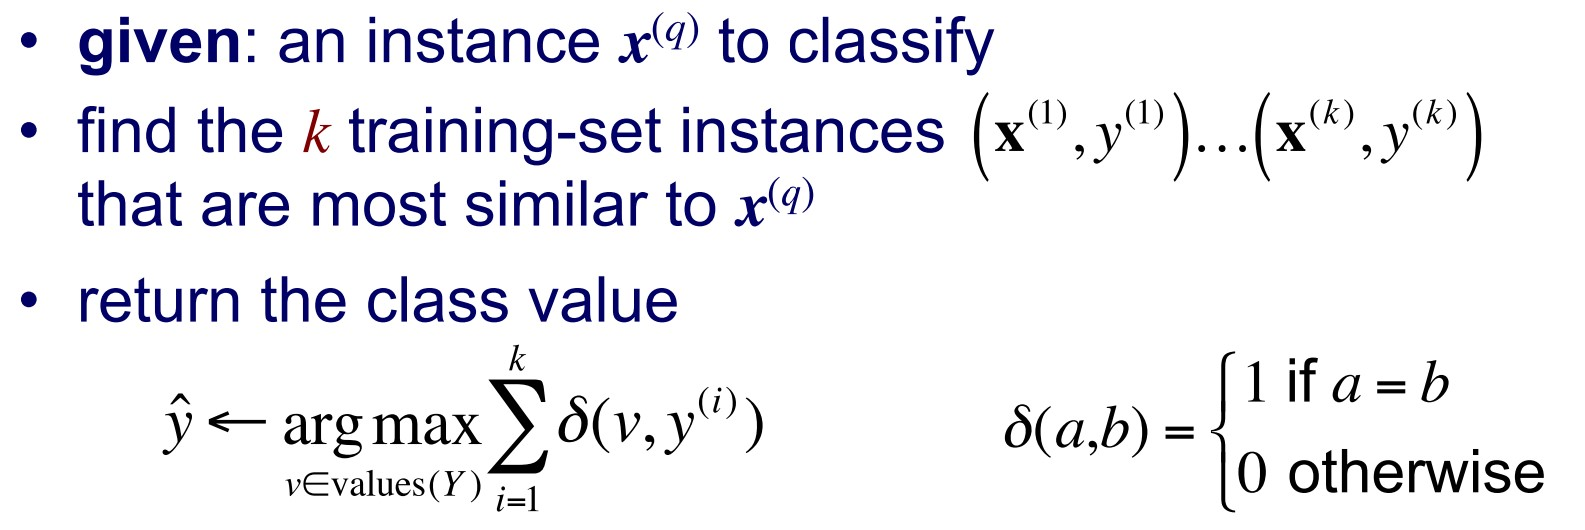
\includegraphics[width=0.7\linewidth]{snips/01_knn-classification.jpg}
    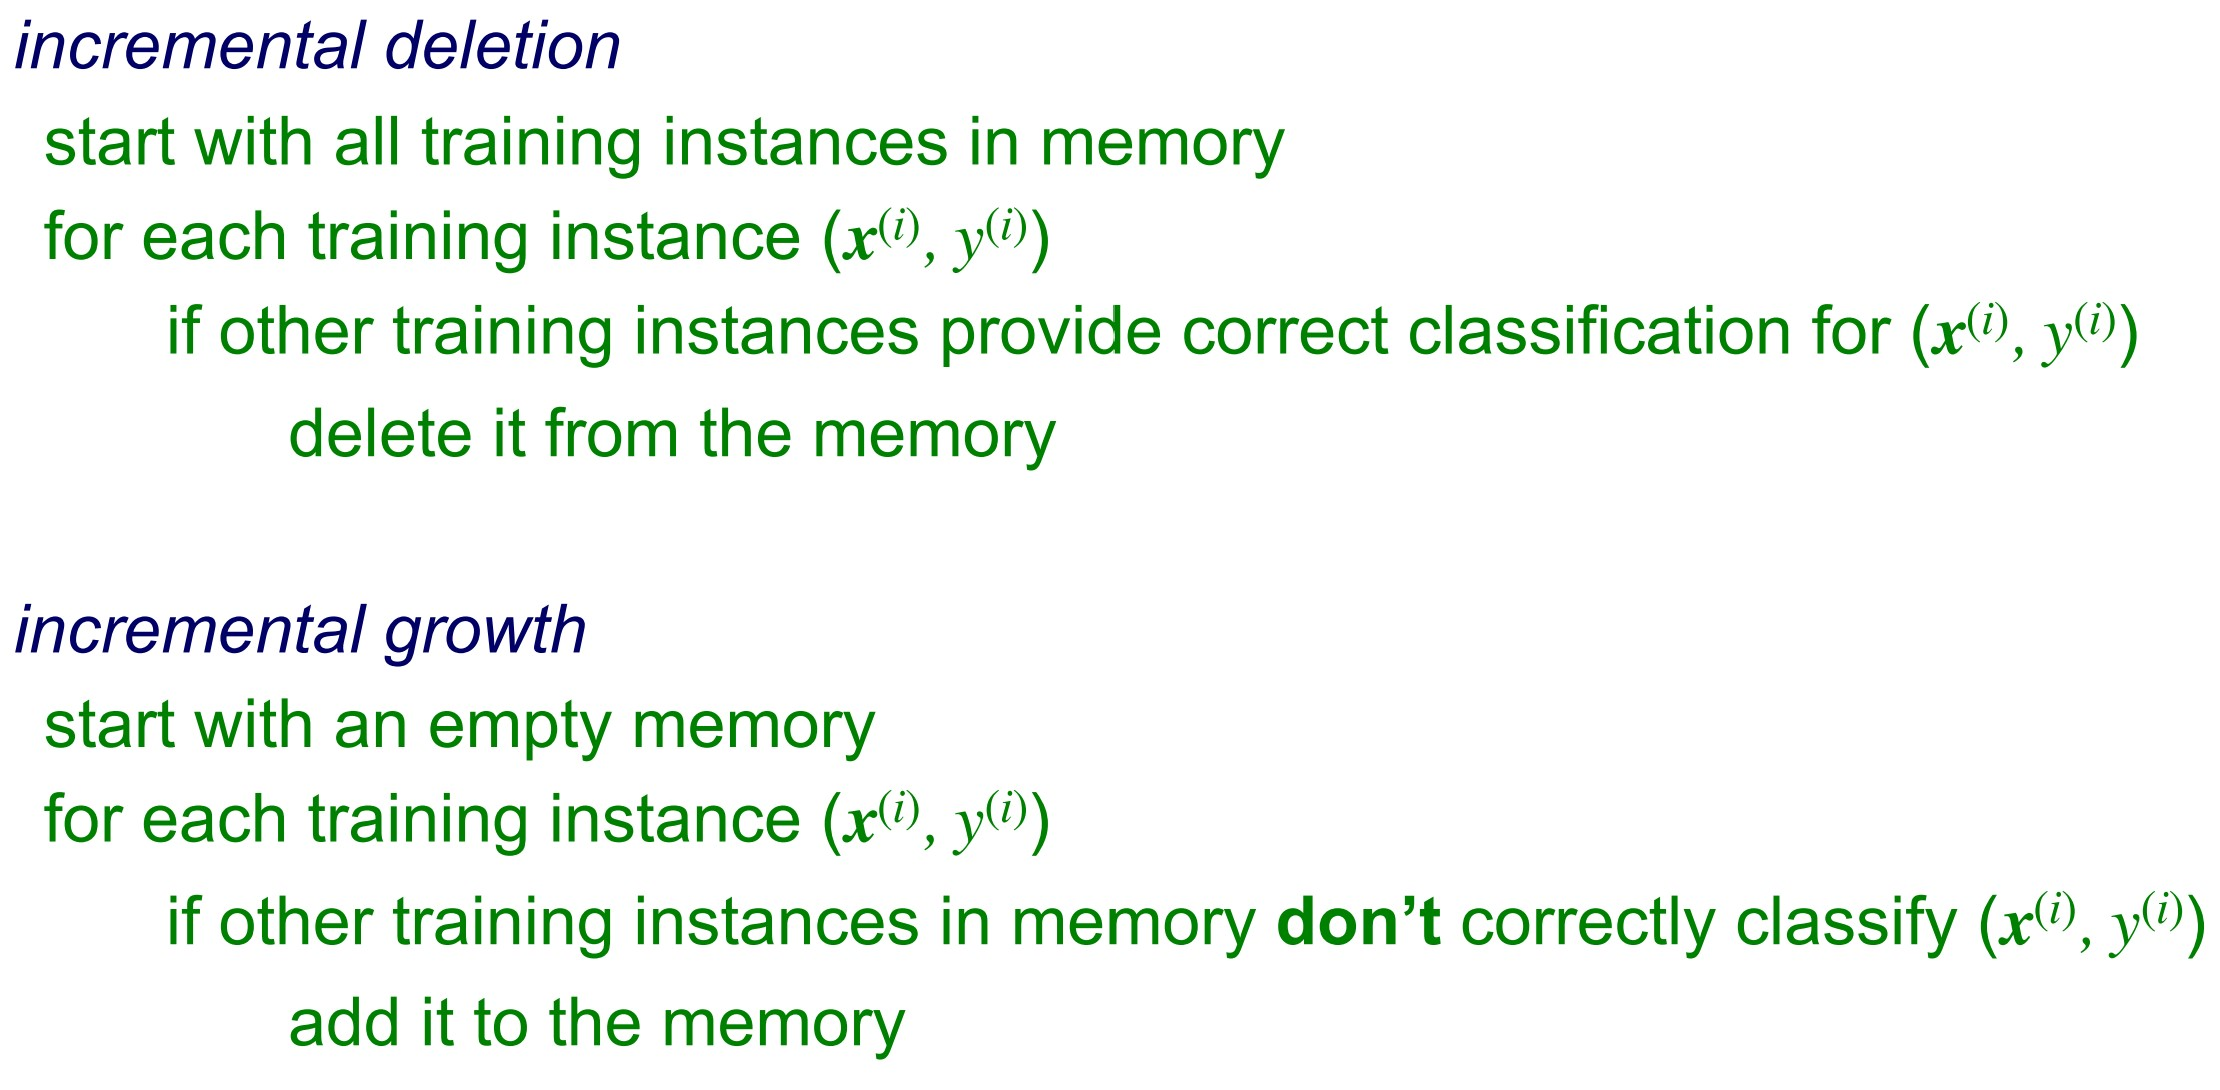
\includegraphics[width=0.9\linewidth]{snips/02_incremental-deletion-and-growth.jpg}

    Find nearest neighbor in k-d tree
    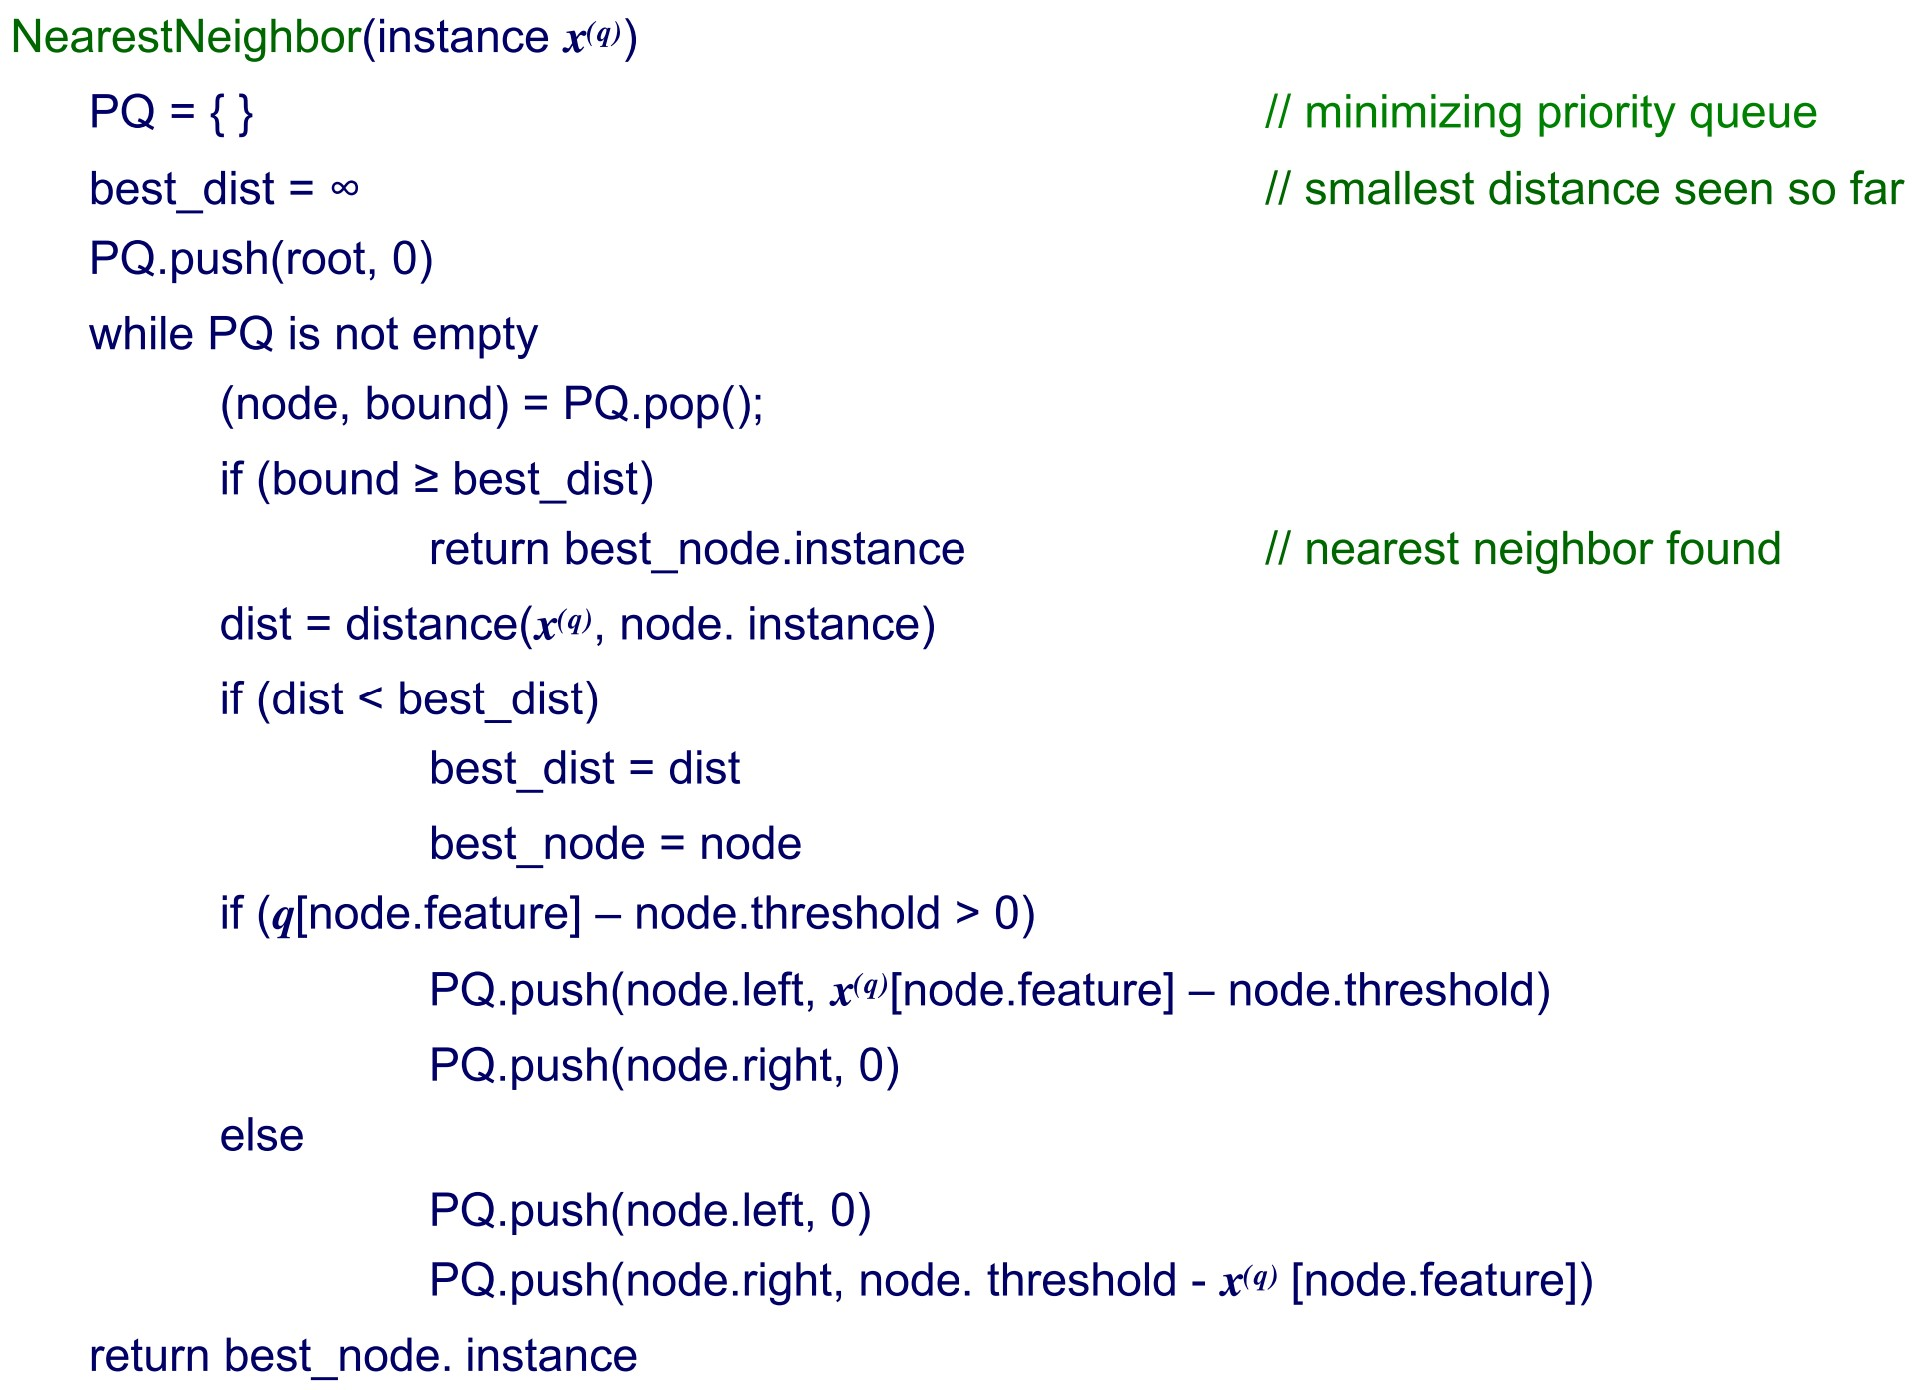
\includegraphics[width=0.9\linewidth]{snips/03_k-d-tree.jpg}

    \section{Decision Trees}
    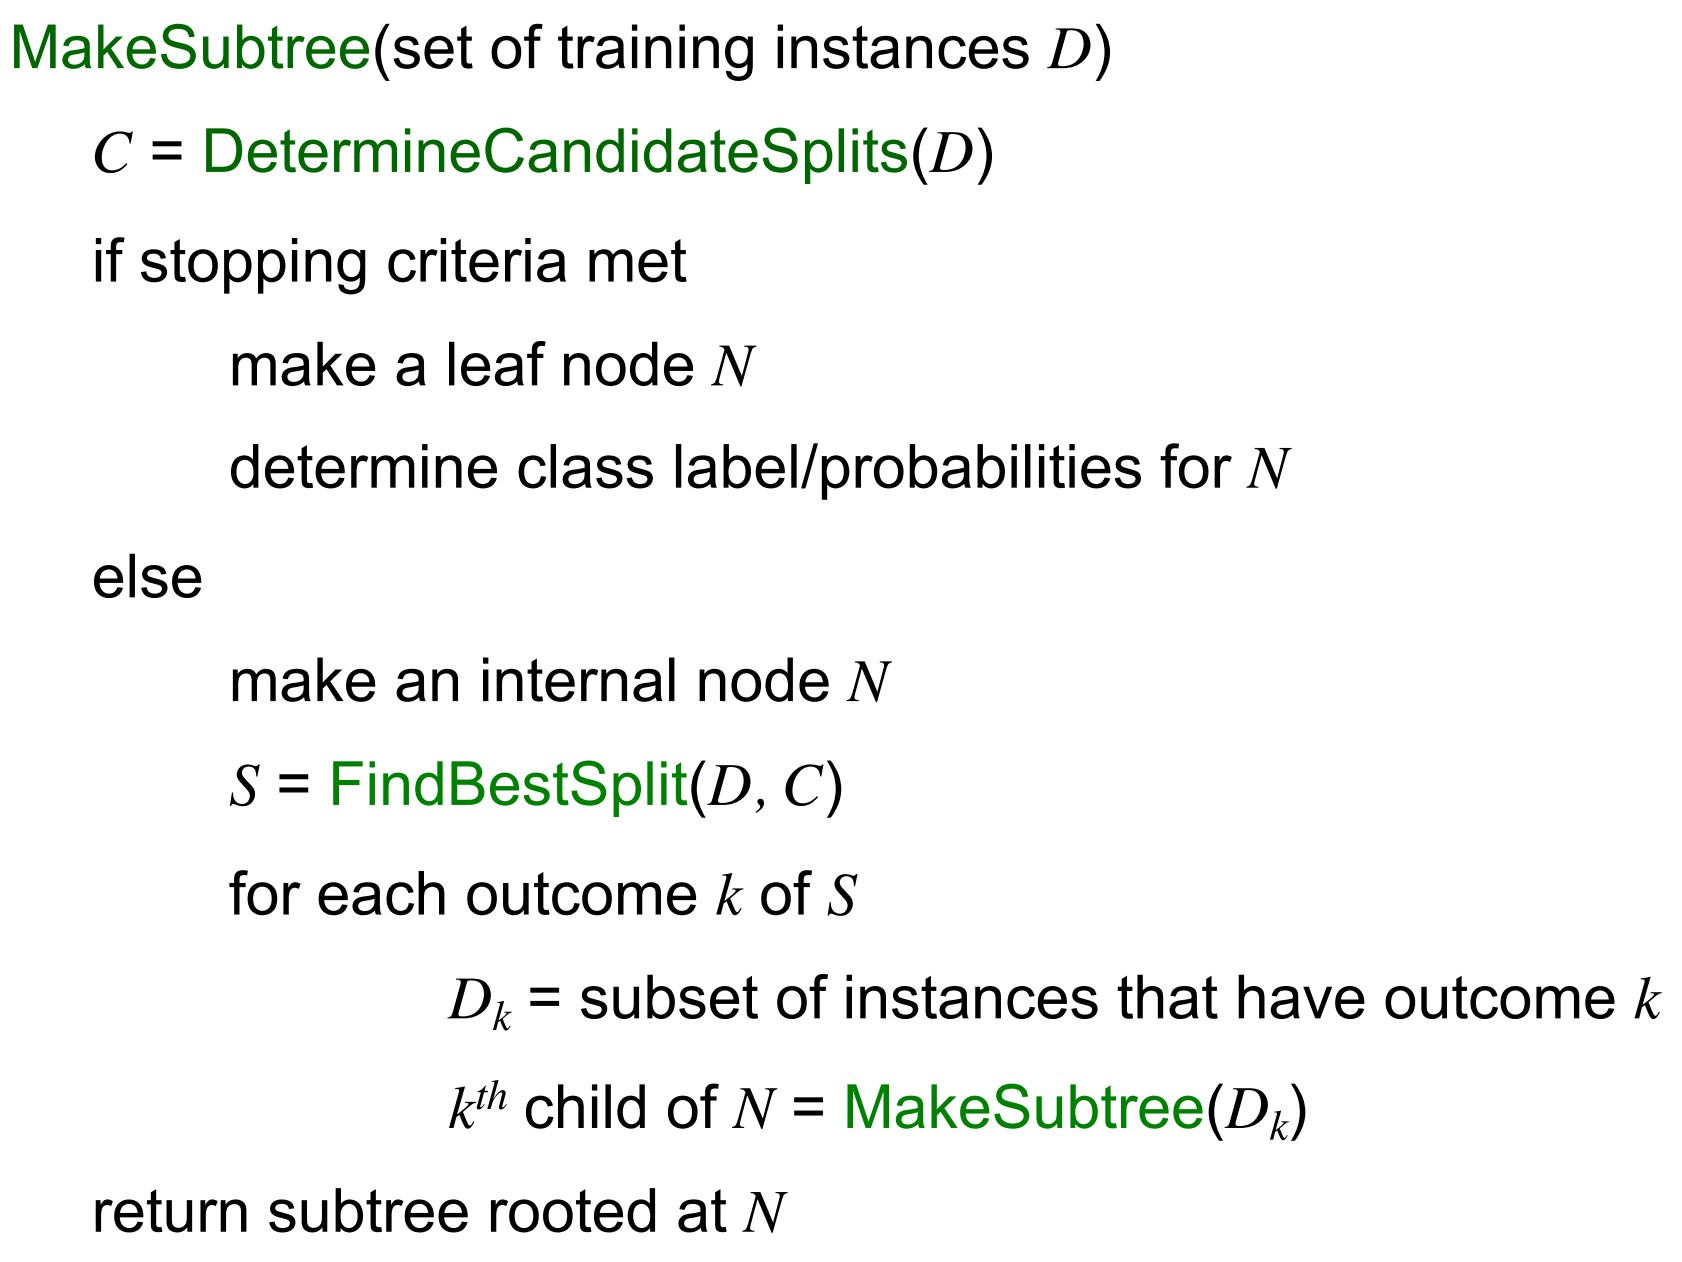
\includegraphics[width=0.8\linewidth]{snips/04_top-down-decision-tree.jpg}
    
    \begin{align*}
        H(Y) &= - \sum_{y} P(y) \log_2 P(y) \\
        H(Y|X) &= \sum_{x} P(X=x) H(Y|X=x) \\
        H(Y|X=x) &= - \sum_{y} P(Y=y|X=x) \log_2 P(Y=y |X=x)
    \end{align*}
    \begin{align*}
        \text{InfoGain}(D,S) &= H_D(Y) - H_D(Y|S) \\
        \text{SplitInfo}(D,S) &= -\sum_{k \in \text{outcomes}(S)} \frac{|D_k|}{|D|} \log_2 \left(  \frac{D_k}{D} \right) \\
        \text{GainRatio} (D,S) &= \frac{\text{InfoGain}(D,S) }{\text{SplitInfo}(D,S) } \\
    \end{align*}
    \begin{equation*}
        \sum_{i=1}^{|D|} (y_i - \hat{y_i})^2 = \sum_{L \in \text{leaves}} \sum_{i\in L} (y_i - \hat{y_i})^2
    \end{equation*}
    Pruning in C4.5

    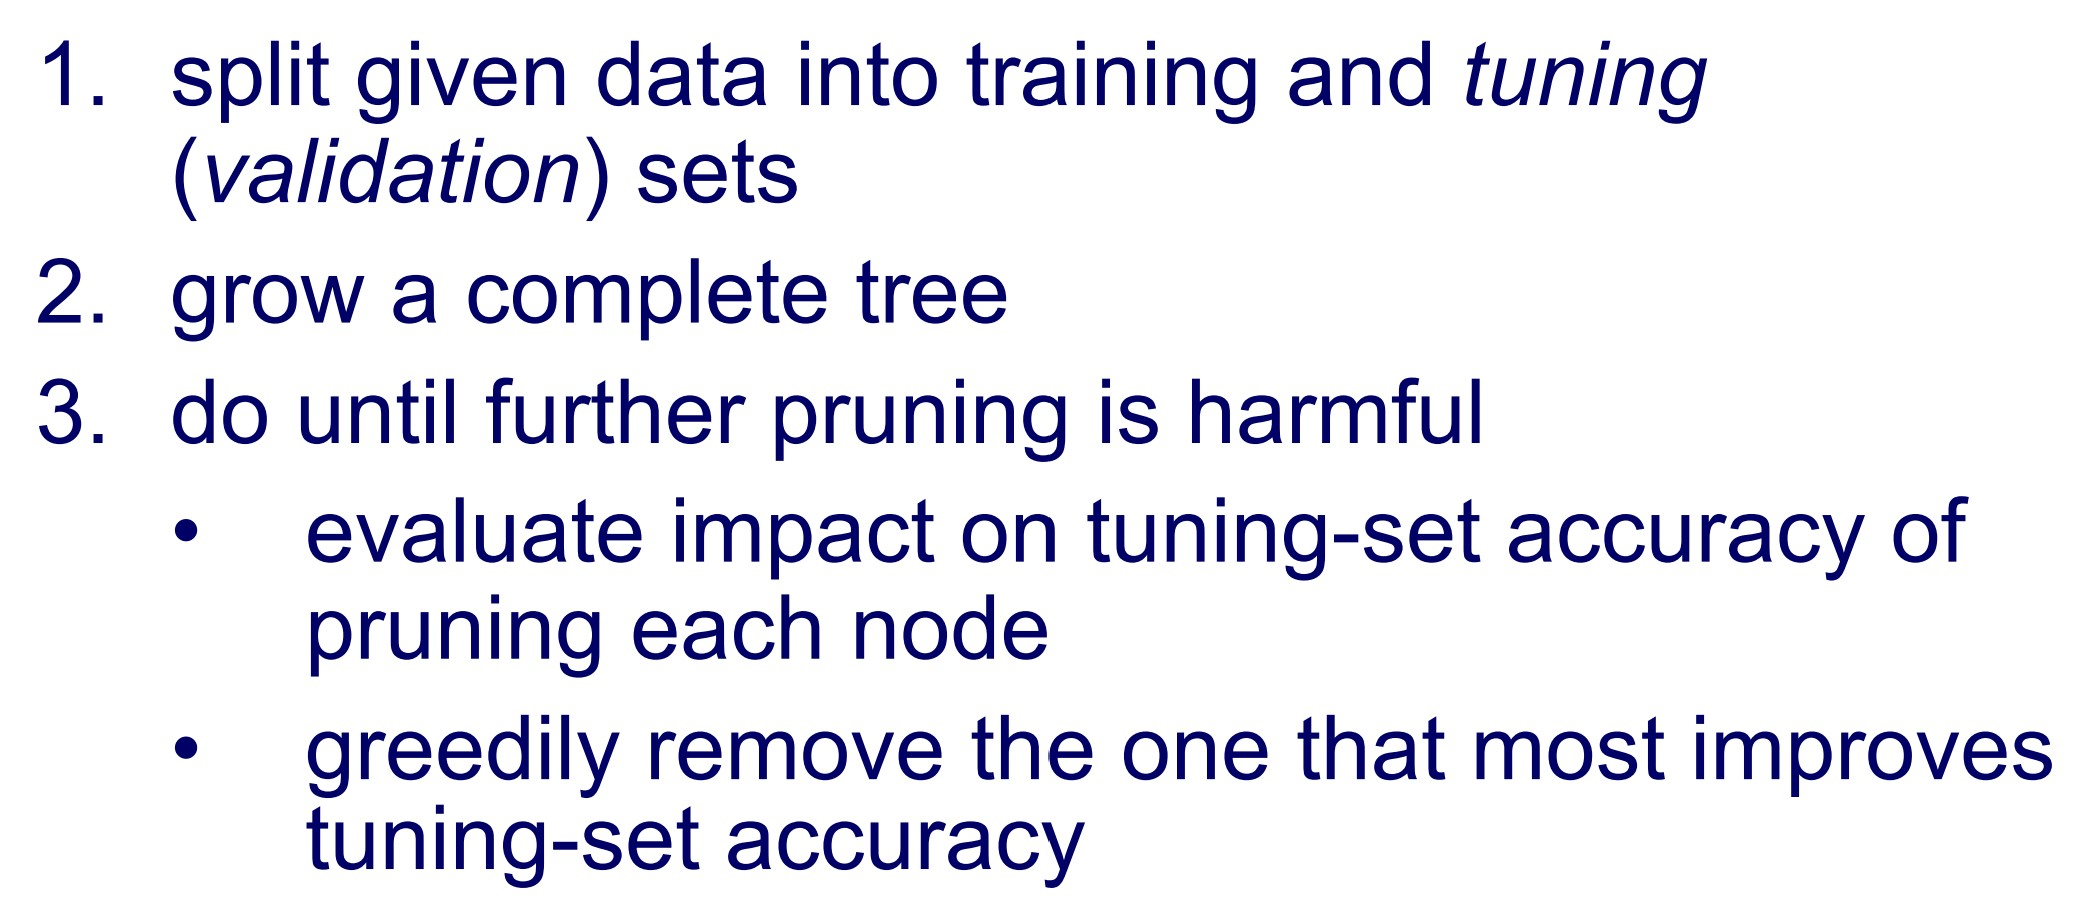
\includegraphics[width=0.65\linewidth]{snips/05_dt-pruning-c45.jpg}
    
    \section{Methodology}
    \begin{align*}
        \text{TPR (recall)} &= \frac{\text{TP}}{\text{TP} + \text{FN}}
        \\
        \text{precision} &= \frac{\text{TP}}{\text{TP}+\text{FP}}
        \\
        \text{FPR} &= \frac{\text{FP}}{\text{TN}+\text{FP}}
    \end{align*}
    \begin{equation*}
        error_D(h) \pm z_{\alpha} \sqrt{\frac{error_D(h)(1 - error_D(h))}{n}}
    \end{equation*}
    \begin{equation*}
        t = \frac{\bar{\delta}}{\sqrt{\frac{1}{n(n-1)}\sum_{i=1}^n (\delta_i - \bar{\delta})^2}}
    \end{equation*}
    Learning curve
    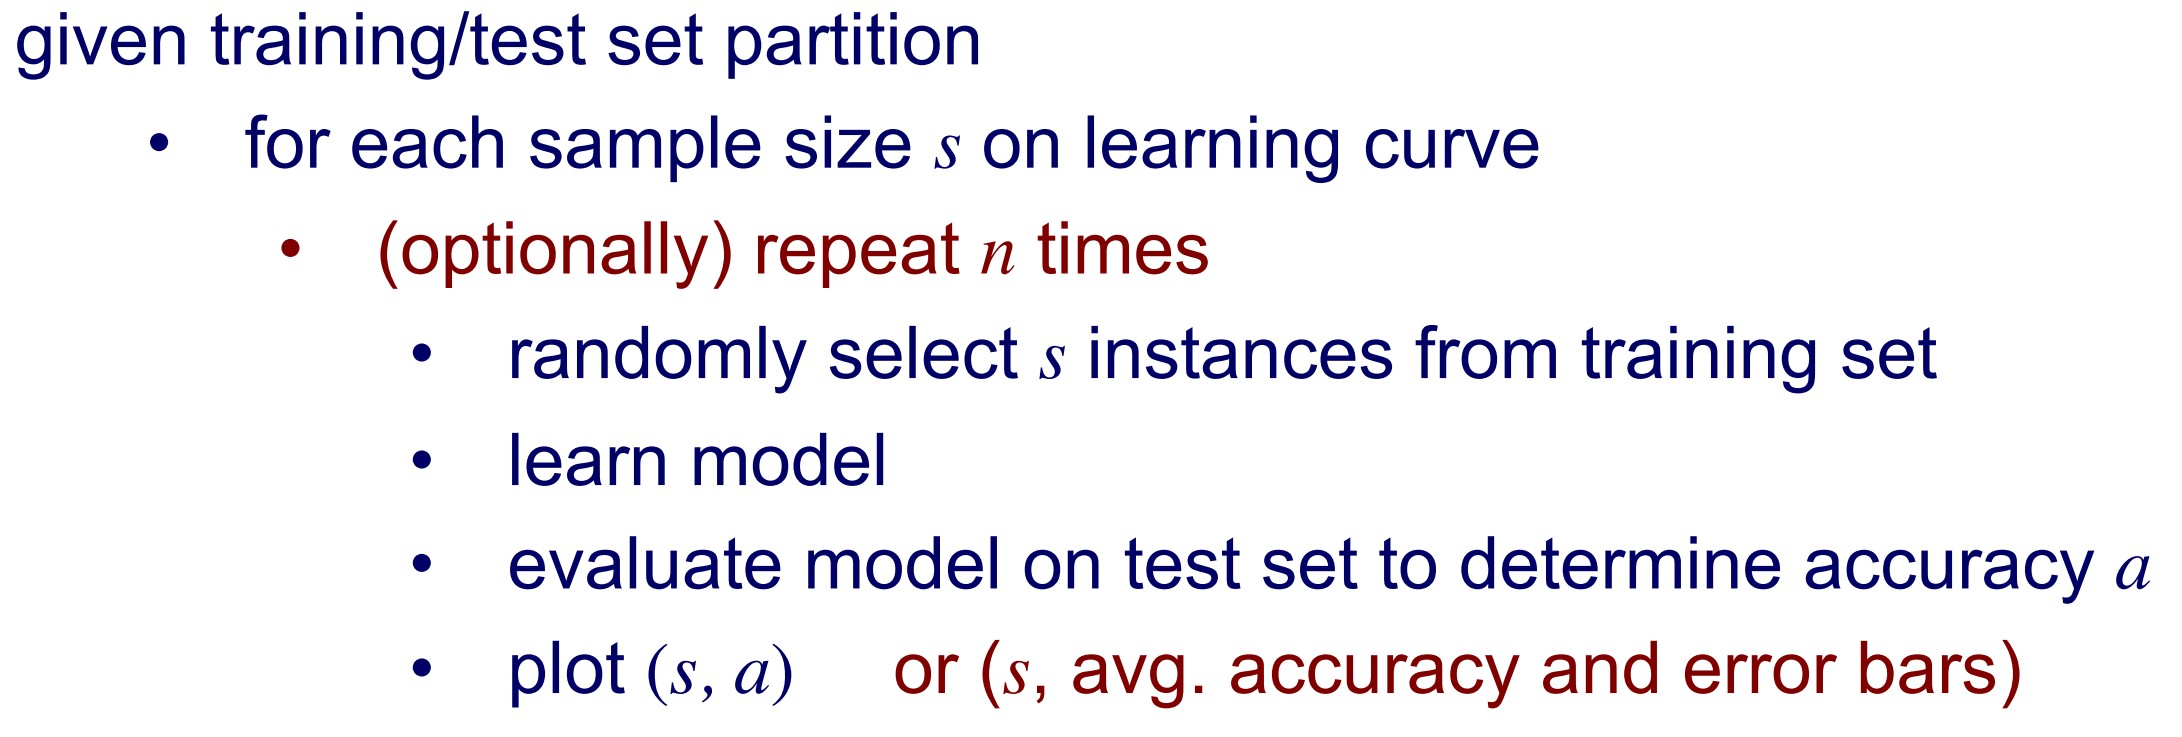
\includegraphics[width=0.8\linewidth]{snips/06_learning-curve.jpg}

    ROC curve
    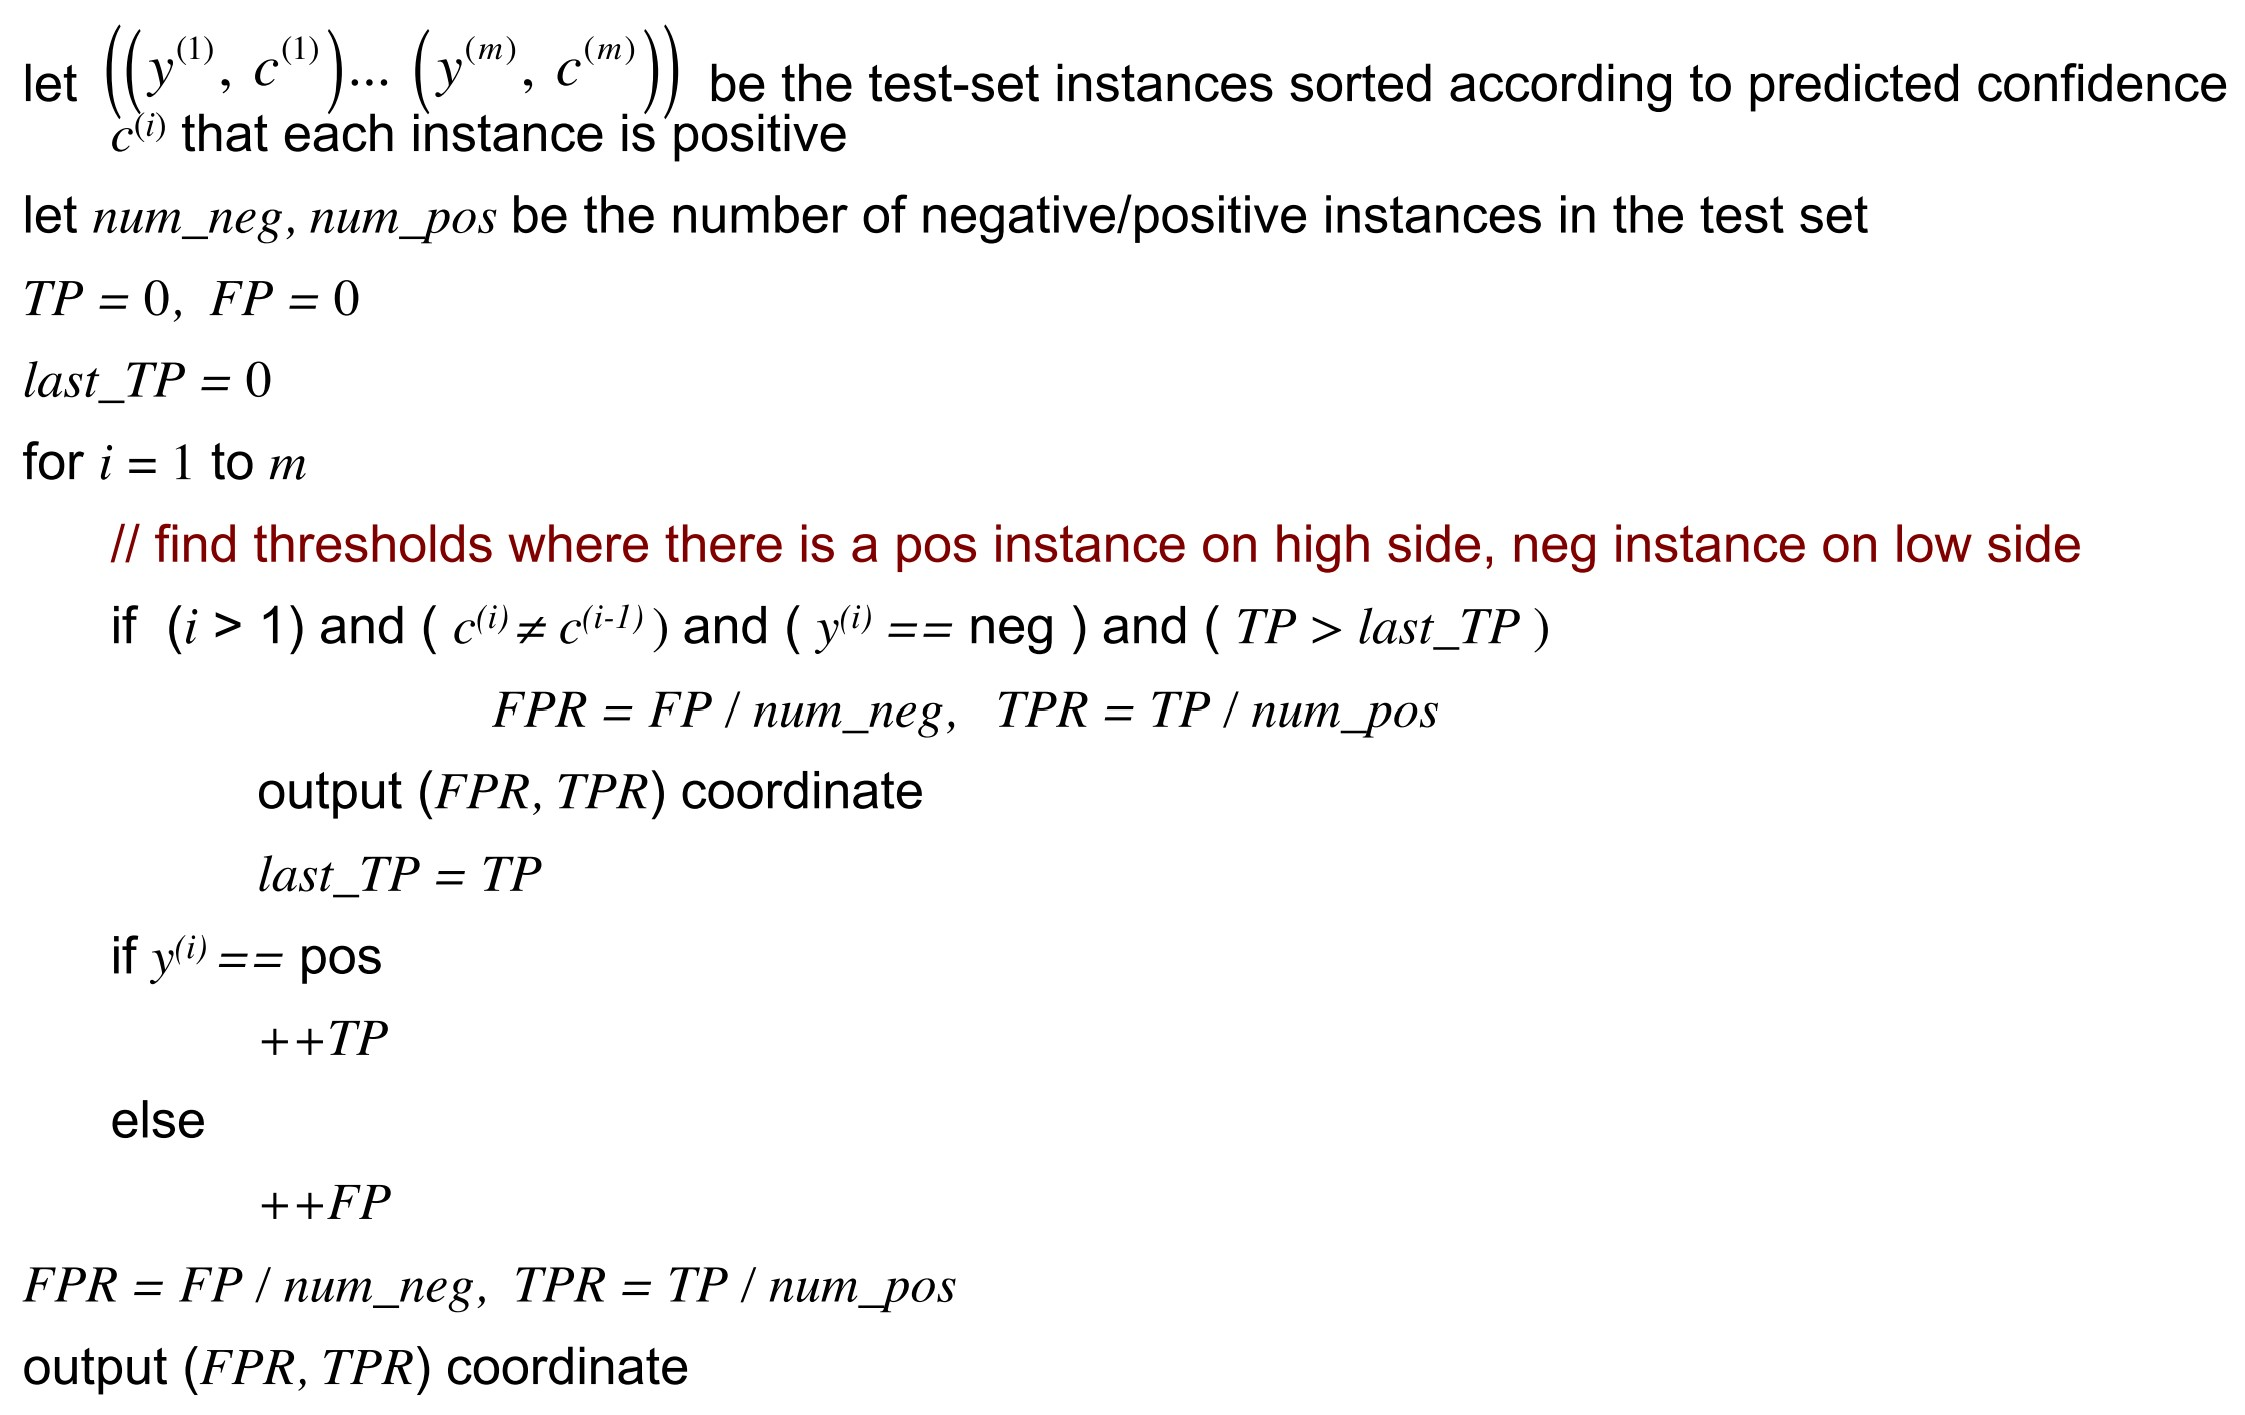
\includegraphics[width=0.9\linewidth]{snips/07_roc-curve.jpg}
    
       
    
    \section{Bayes Network}
    
    \begin{equation*}
        P(X_1, \dots,X_n) = \prod_{i=1}^n P(X_i | \text{Parents}(X_i))
    \end{equation*}
    \begin{equation*}
        P(b|j,m) = \frac{P(b,j,m)}{P(j,m)} = \frac{P(b,j,m)}{P(b,j,m) + P(\neg b,j,m)}
    \end{equation*}
    \begin{equation*}
        \text{MAP (Laplace): } P(X=x) = \frac{n_x+1}{\sum_{v \in \text{values}(X)} (n_v+1)}
    \end{equation*}
    \begin{equation*}
        \text{m-estimates: } P(X=x) = \frac{n_x+p_xm}{\left(\sum_{v \in \text{values}(X)} n_v \right) + m}
    \end{equation*}
    \begin{equation*}
        \text{M-step: } P(a|b,e) = \frac{E\#(a \wedge b \wedge e)}{E\#( b \wedge e)}
    \end{equation*}
    \begin{equation*}
        I(X,Y) = \sum_{x} \sum_{y} P(x,y) \log_2 \frac{P(x,y)}{P(x)P(y)}
    \end{equation*}
    \begin{equation*}
        P(X_1,\dots,X_n,Y) = P(Y) \prod_{i=1}^n P(X_i|Y)
    \end{equation*}
    \begin{equation*}
        P(Y=y|X) = \frac{P(y)\prod_{i=1}^n P(x_i|y)}{\sum_{y'} P(y')\prod_{i=1}^n P(x_i|y')}
    \end{equation*}
    \begin{equation*}
        I(X_i,X_j|Y) = \sum_{x_i} \sum_{x_j} \sum_{y}  P(x_i,x_y,y) \log_2 \frac{P(x_i,x_j|y)}{P(x_i|y)P(x_j|y)}
    \end{equation*}
    \begin{equation*}
        P(Y=y|\bold{x}) = \frac{P(y)P(\bold{x}|y)}{\sum_{y'}P(y')P(\bold{x}|y')}
    \end{equation*}
    MCMC Gibbs Sampling
    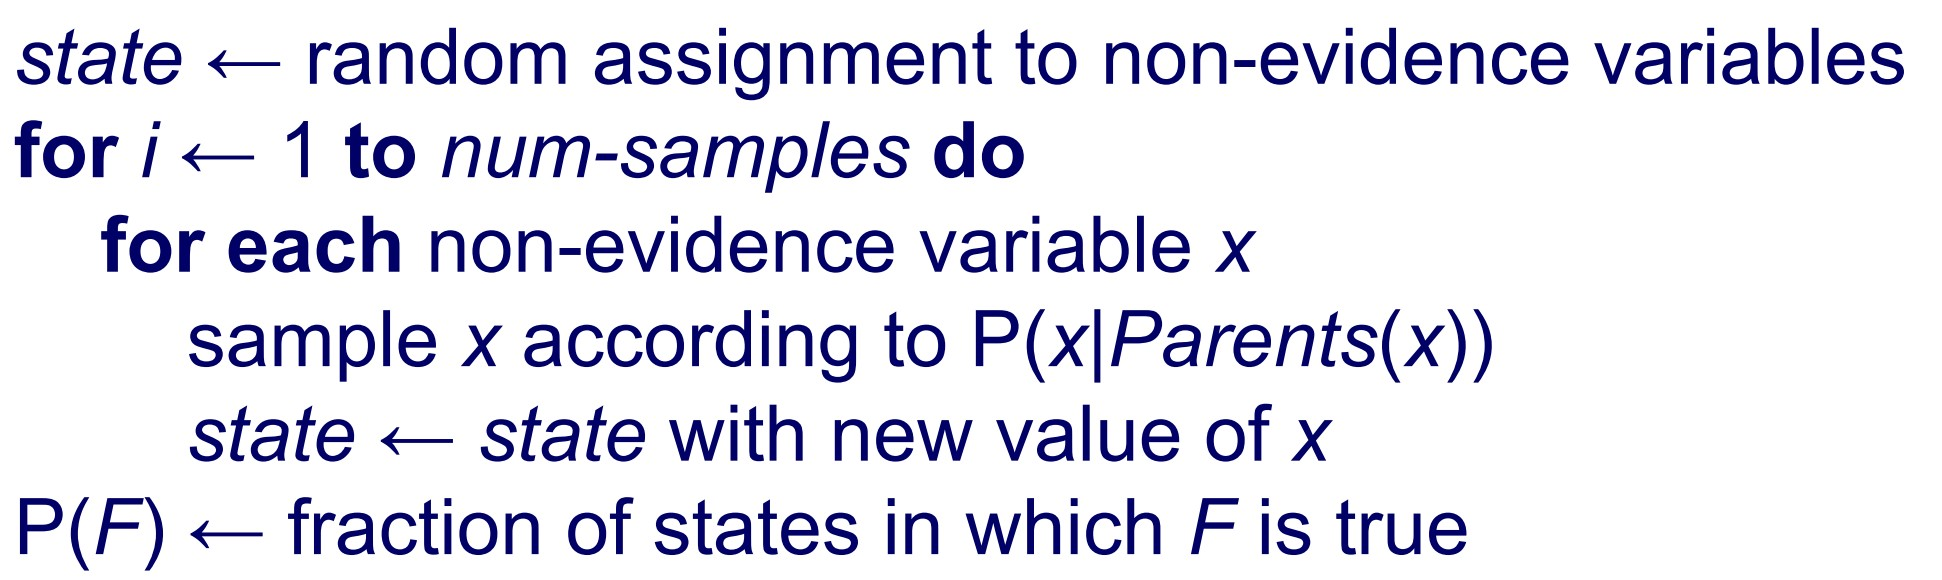
\includegraphics[width=0.7\linewidth]{snips/08_mcmc-gibbs.jpg}

    EM algorithm
    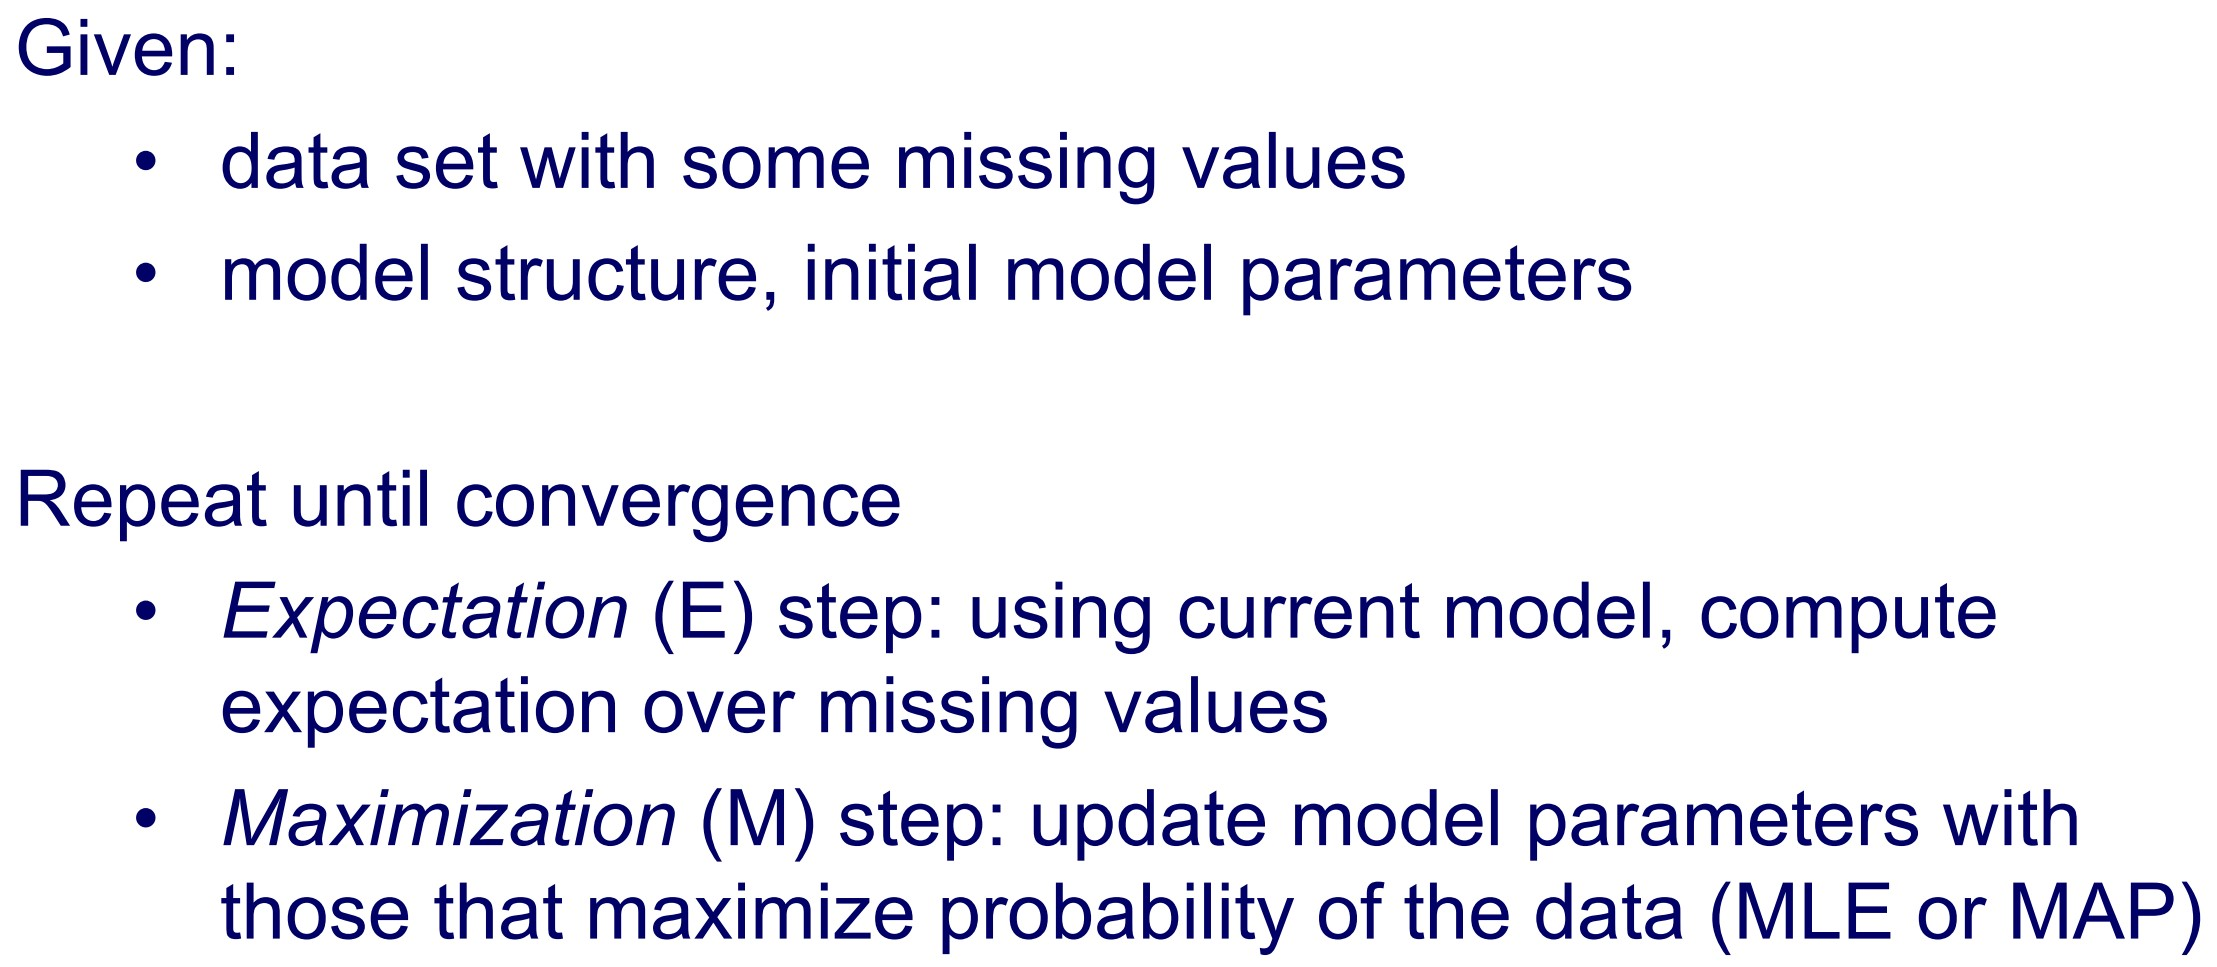
\includegraphics[width=0.8\linewidth]{snips/09_EM-bayes-net.jpg}
    
    Chow-Liu

    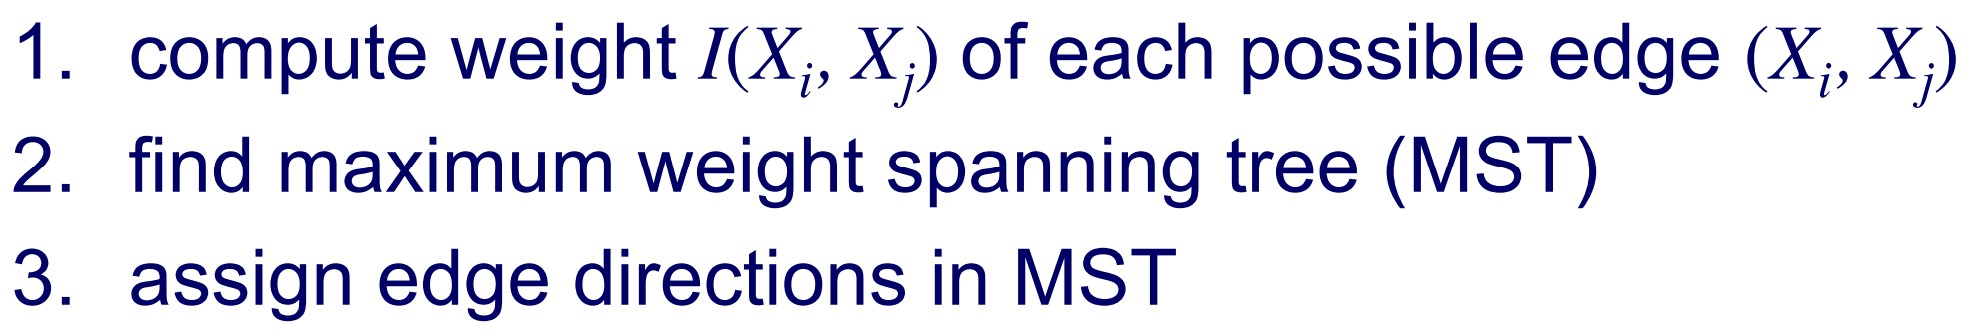
\includegraphics[width=0.7\linewidth]{snips/10_chow-liu.jpg}
    
    Prim MST
    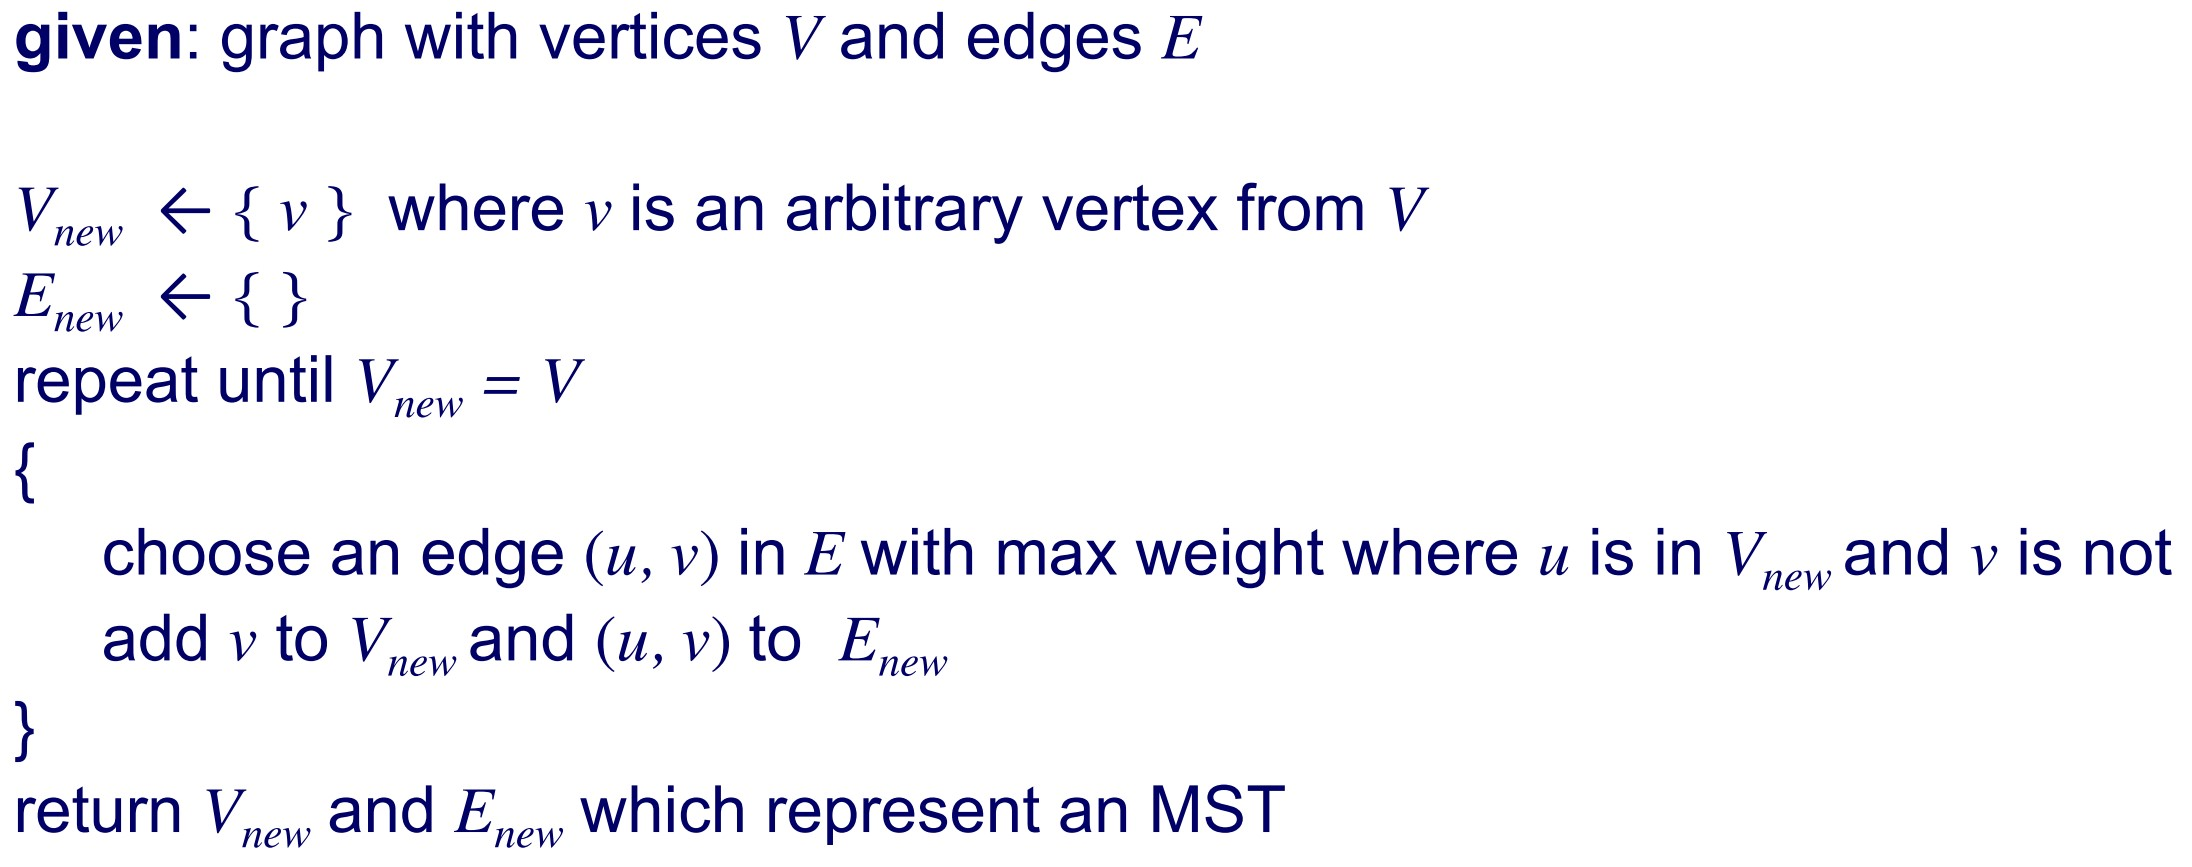
\includegraphics[width=0.9\linewidth]{snips/11_prim-mst.jpg}
    
    Kruskal MST

    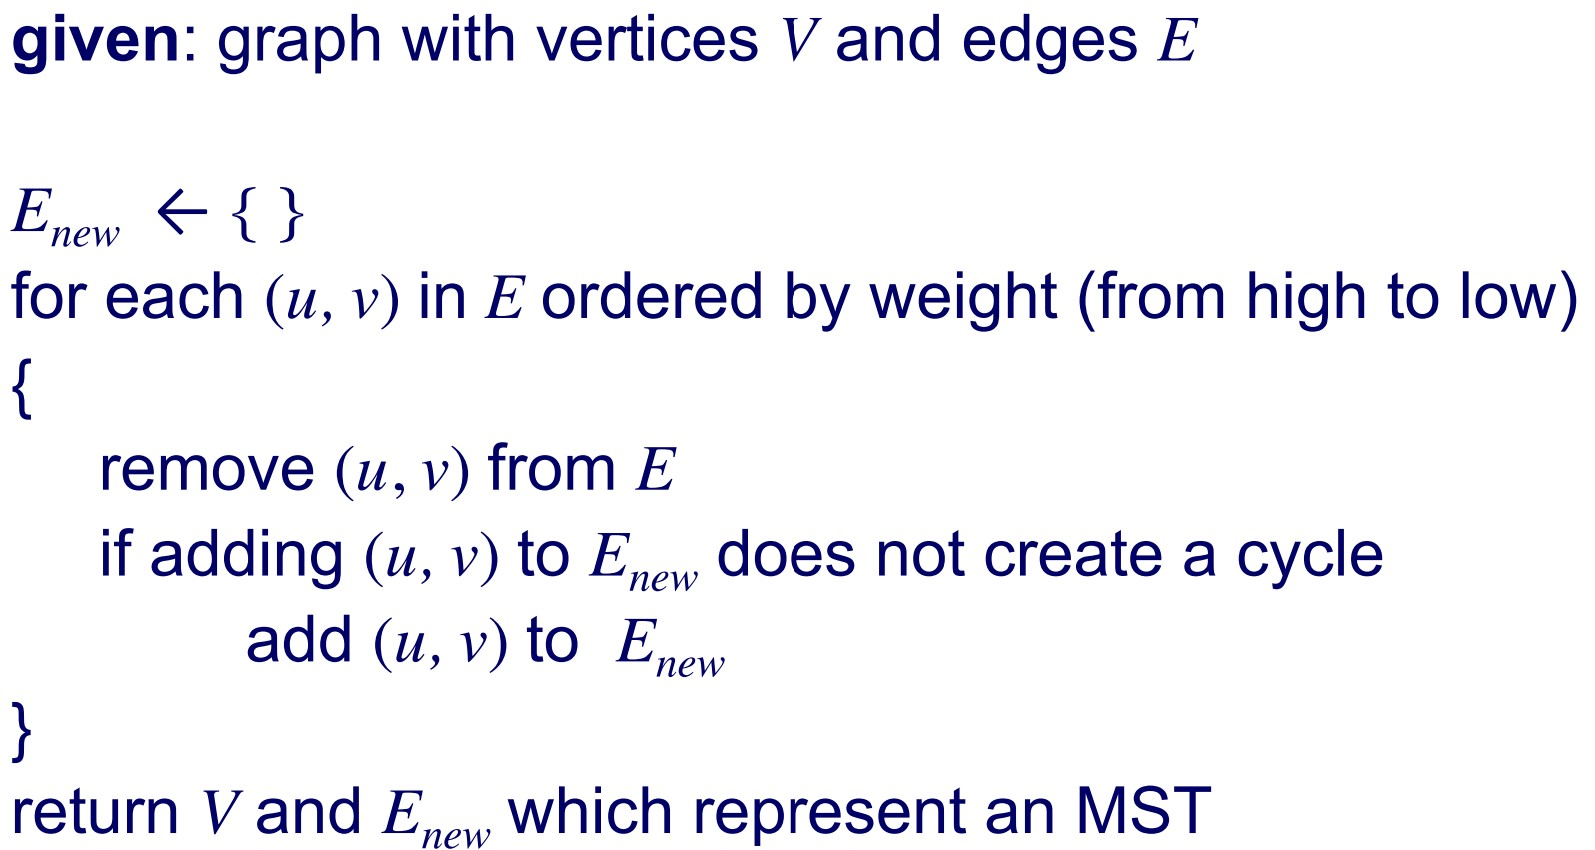
\includegraphics[width=0.7\linewidth]{snips/12_kruskal-mst.jpg}
    
    BN Hill Climbing Algorithm
    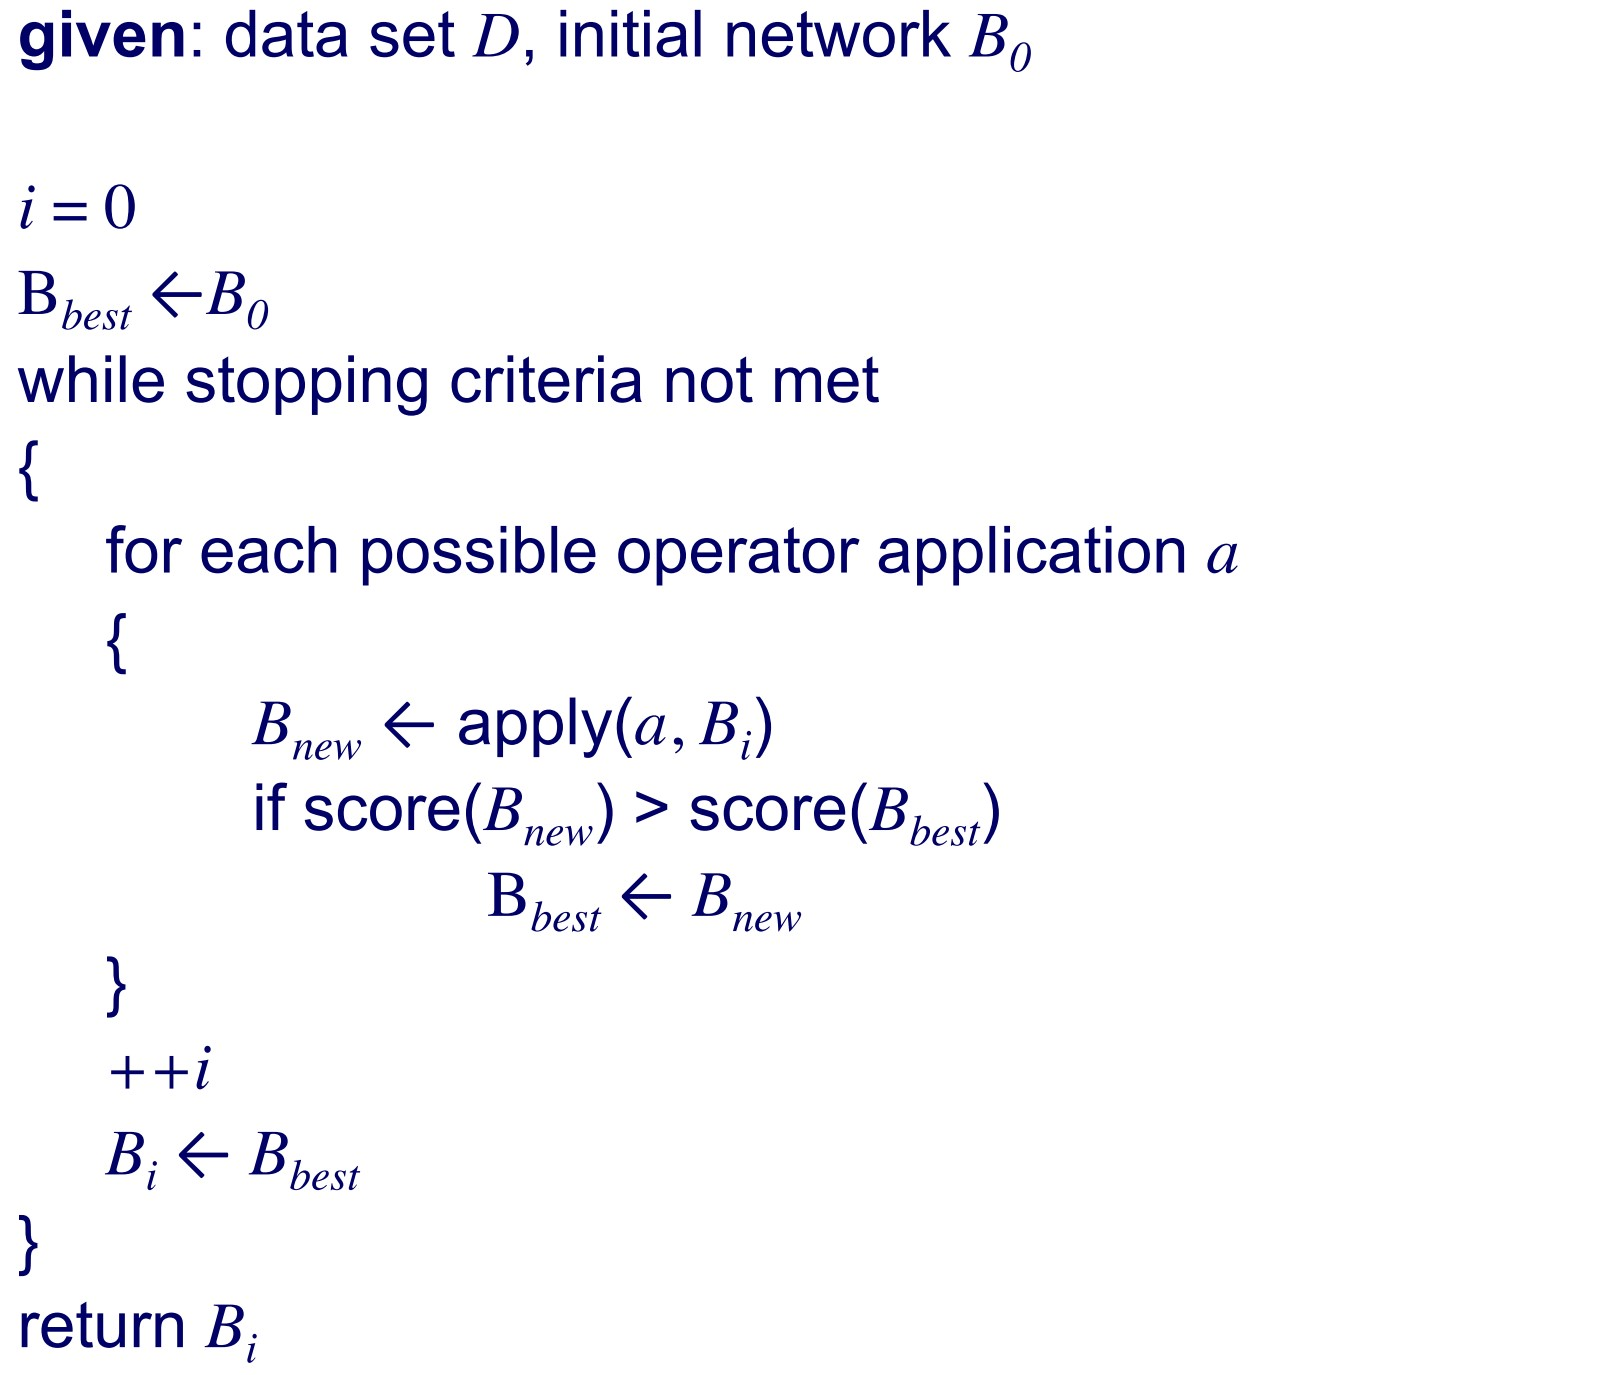
\includegraphics[width=0.7\linewidth]{snips/13_bn-hill-climb.jpg}
    
    TAN algorithm
    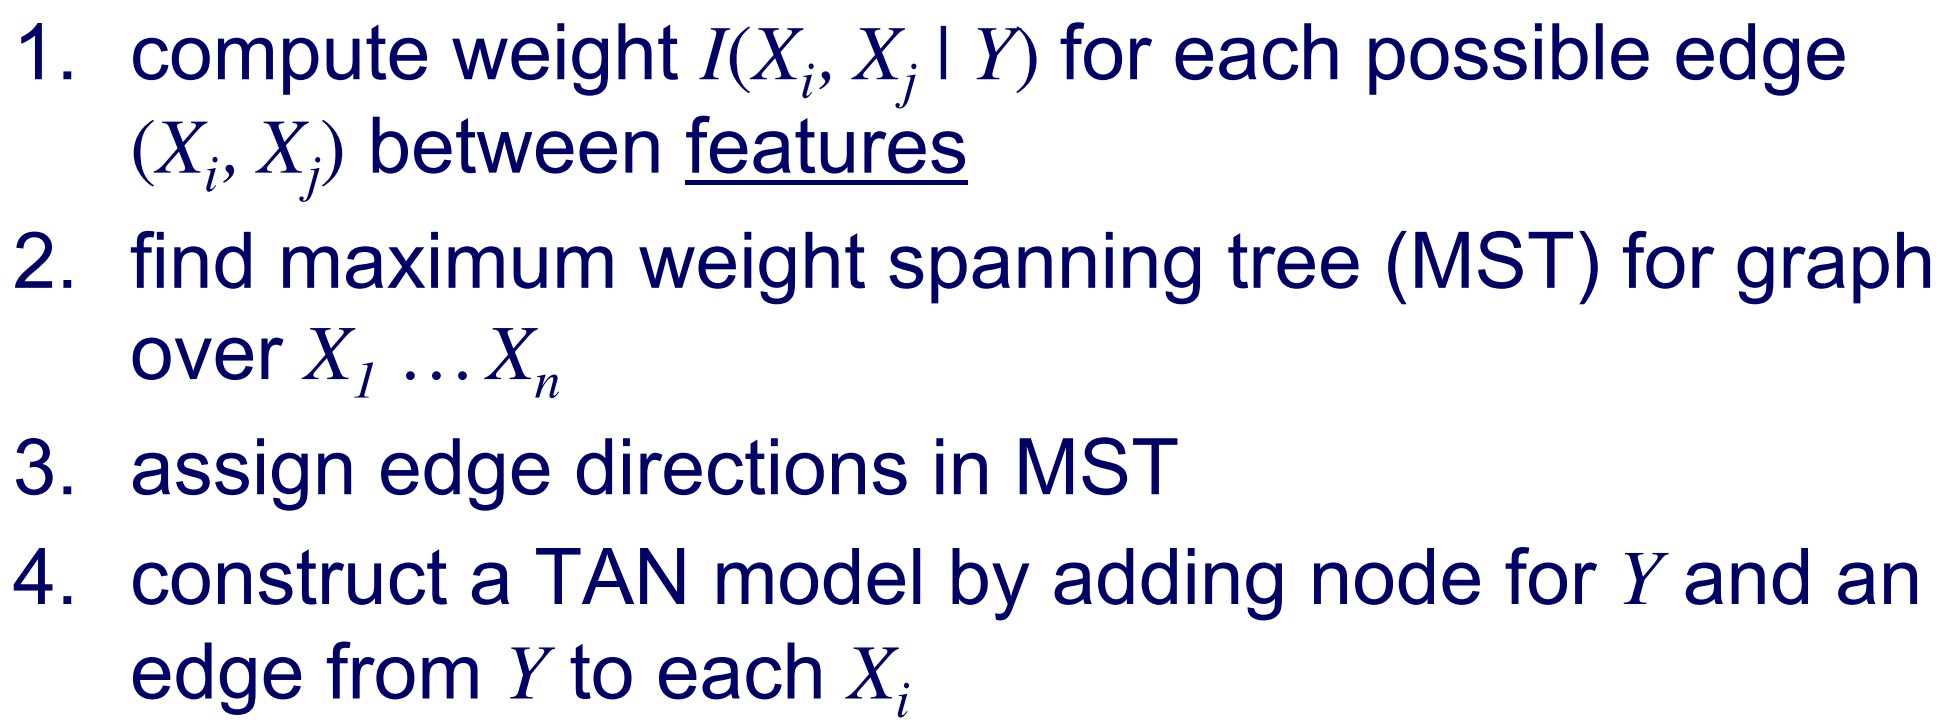
\includegraphics[width=0.7\linewidth]{snips/14_tan.jpg}
    
    
    \section{Markov Network}
    
    \begin{equation*}
        P(\bold{V}) = \frac{1}{Z} \prod_k \phi_k(\bold{V})
    \end{equation*}
    \begin{equation*}
        Z = \sum_{\bold{v} \in \bold{V}} \prod_k \phi_k(\bold{v})
    \end{equation*}
    
    
    \section{Neural Network}
    
    \begin{align*}
        E(\bold{w}) &= \frac{1}{2} \sum_{d \in D} \left(y^{(d)} - o^{(d)} \right)^2
        \\
        E(\bold{w}) &= \sum_{d \in D} - y^{(d)} \ln \left( o^{(d)}\right) - \left(1 - y^{(d)}\right) \ln \left( 1-o^{(d)} \right)
        \\
        E(\bold{w}) &= -\sum_{d \in D} \sum_{i=1}^{\#class} y_i^{(d)} \ln \left( o_i^{(d)}\right)
    \end{align*}
    \begin{equation*}
        net = w_0 + \sum_i w_i x_i
    \end{equation*}
    \begin{align*}
        f(net) &= \frac{1}{1 + e^{-net}}
        & \text{(Sigmoid)}
        \\
        f(net) &= \tanh(x) = \frac{2}{1+e^{-2net}} - 1
        & \text{(Tanh)}
        \\
        f(net) &= 
        \begin{cases} 
            0 \quad \text{if } x < 0 \\ 
            x \quad \text{if } x \geq 0 
        \end{cases}
        & \text{(ReLU)}
        \\
        f(net) &= \frac{e^{net_j}} {\sum_j e^{net_j}}
        & \text{(softmax)}
    \end{align*}
    \begin{equation*}
        \Delta \bold{w} = - \eta \nabla_\bold{w} E(\bold{w})
    \end{equation*}
    \begin{equation*}
        \Delta w_{ji} = \eta \delta_j o_i
    \end{equation*}
    \begin{equation*}
        \delta_j = - \frac{\partial E}{\partial net_j} = \text{e.g.} \; o_j (1-o_j) \sum_k \delta_k w_{kj}
    \end{equation*}

	NNet Optimization (1 = velocity, 2 = nesterov)
    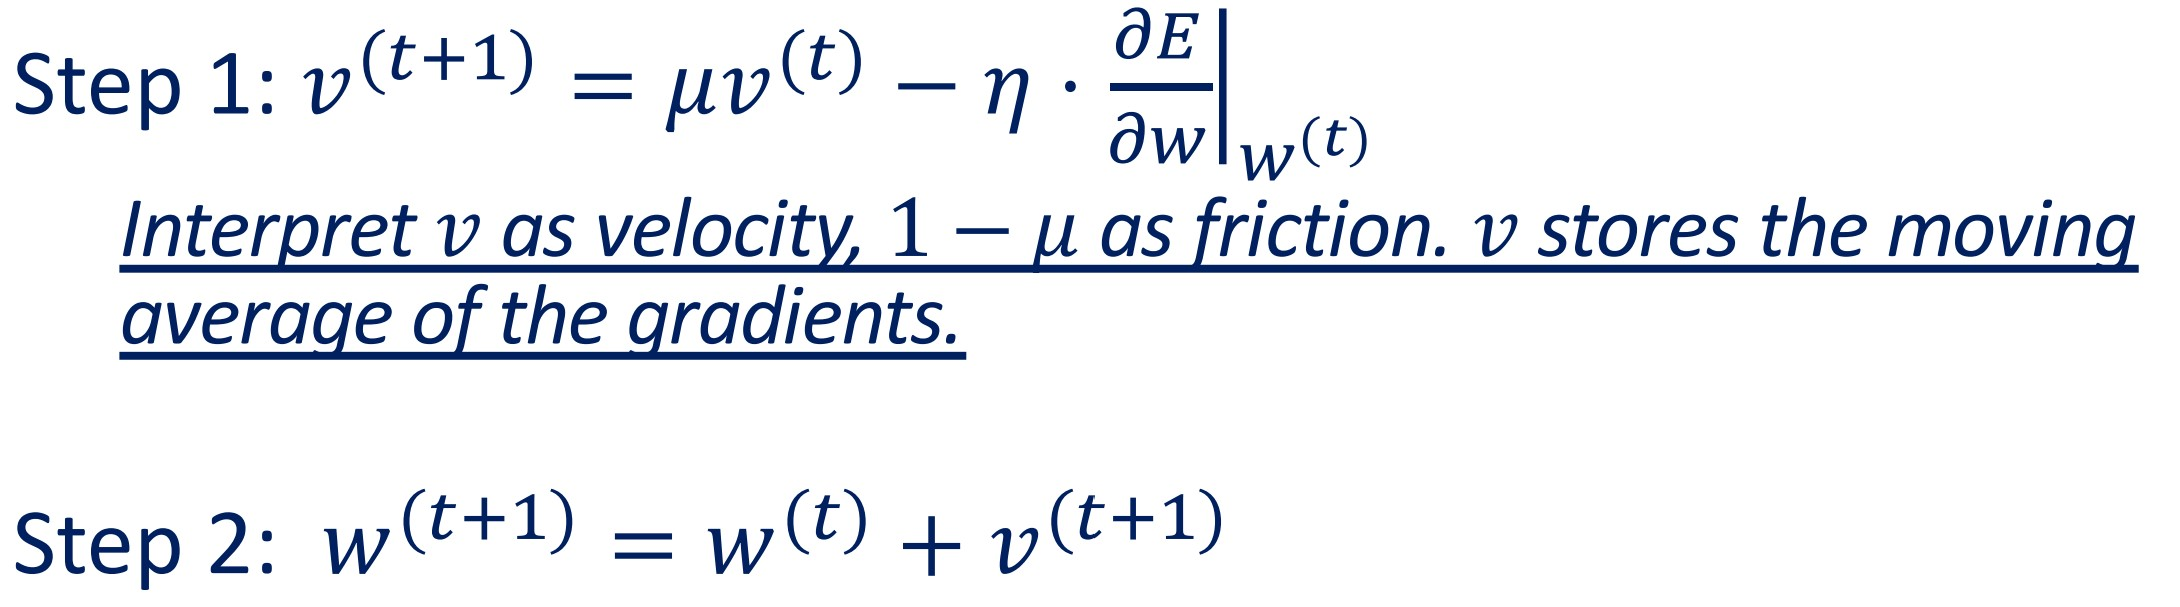
\includegraphics[width=0.7\linewidth]{snips/16_momentum.jpg}
    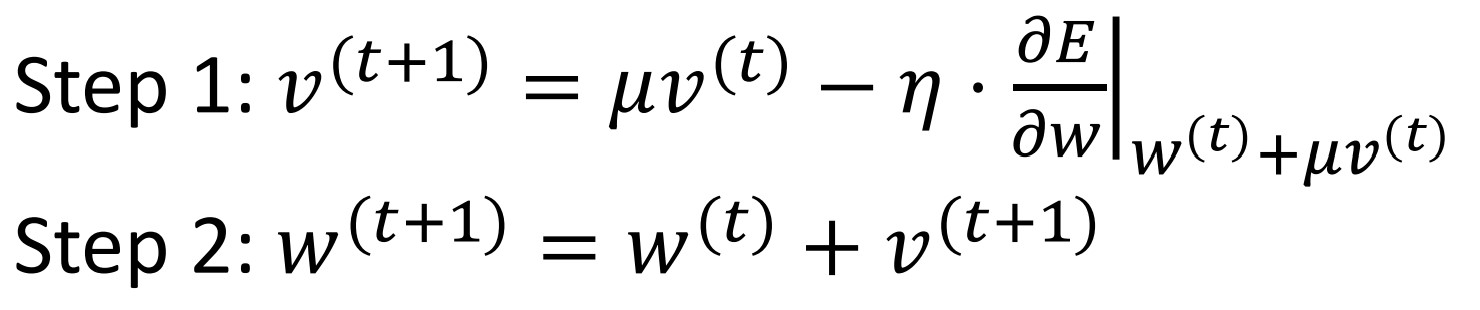
\includegraphics[width=0.55\linewidth]{snips/17_nesterov-accelerated.jpg}
    
    % GAN
    \begin{align*}
        E \left(\theta^{(D)} \right) = &- \frac{1}{2} E_{x \sim p_{data}} \log D(\bold{x}) \\
        &- \frac{1}{2} E_{z} \log \left(1 - D(G(\bold{z})) \right) \\
    % \end{align*}
    % \begin{align*}    
        E \left(\theta^{(G)} \right) = &- E \left(\theta^{(D)} \right)
    \end{align*}
    \begin{align*}
        \min_G \max_D E_{x \sim p_{data}} \log D(\bold{x}) + E_{z} \log \left(1 - D(G(\bold{z})) \right) \\
    \end{align*}
    
    
    \section{Linear Models}
    
    % \begin{align*}
    %     E(\bold{\beta}) = || \bold{y} - X \bold{\beta} ||_2^2  + \lambda ||\bold{\beta}||_2^2
    % \end{align*}
    Ridge regression
    \begin{align*}
        \hat{\beta} = \left(X^TX - \lambda I \right)^{-1} X^T Y
    \end{align*}
    % \begin{align*}
    %     E(\bold{\beta}) = || \bold{y} - X \bold{\beta} ||_2^2  + \lambda ||\bold{\beta}||_1
    % \end{align*}

    LASSO coordinate descent
    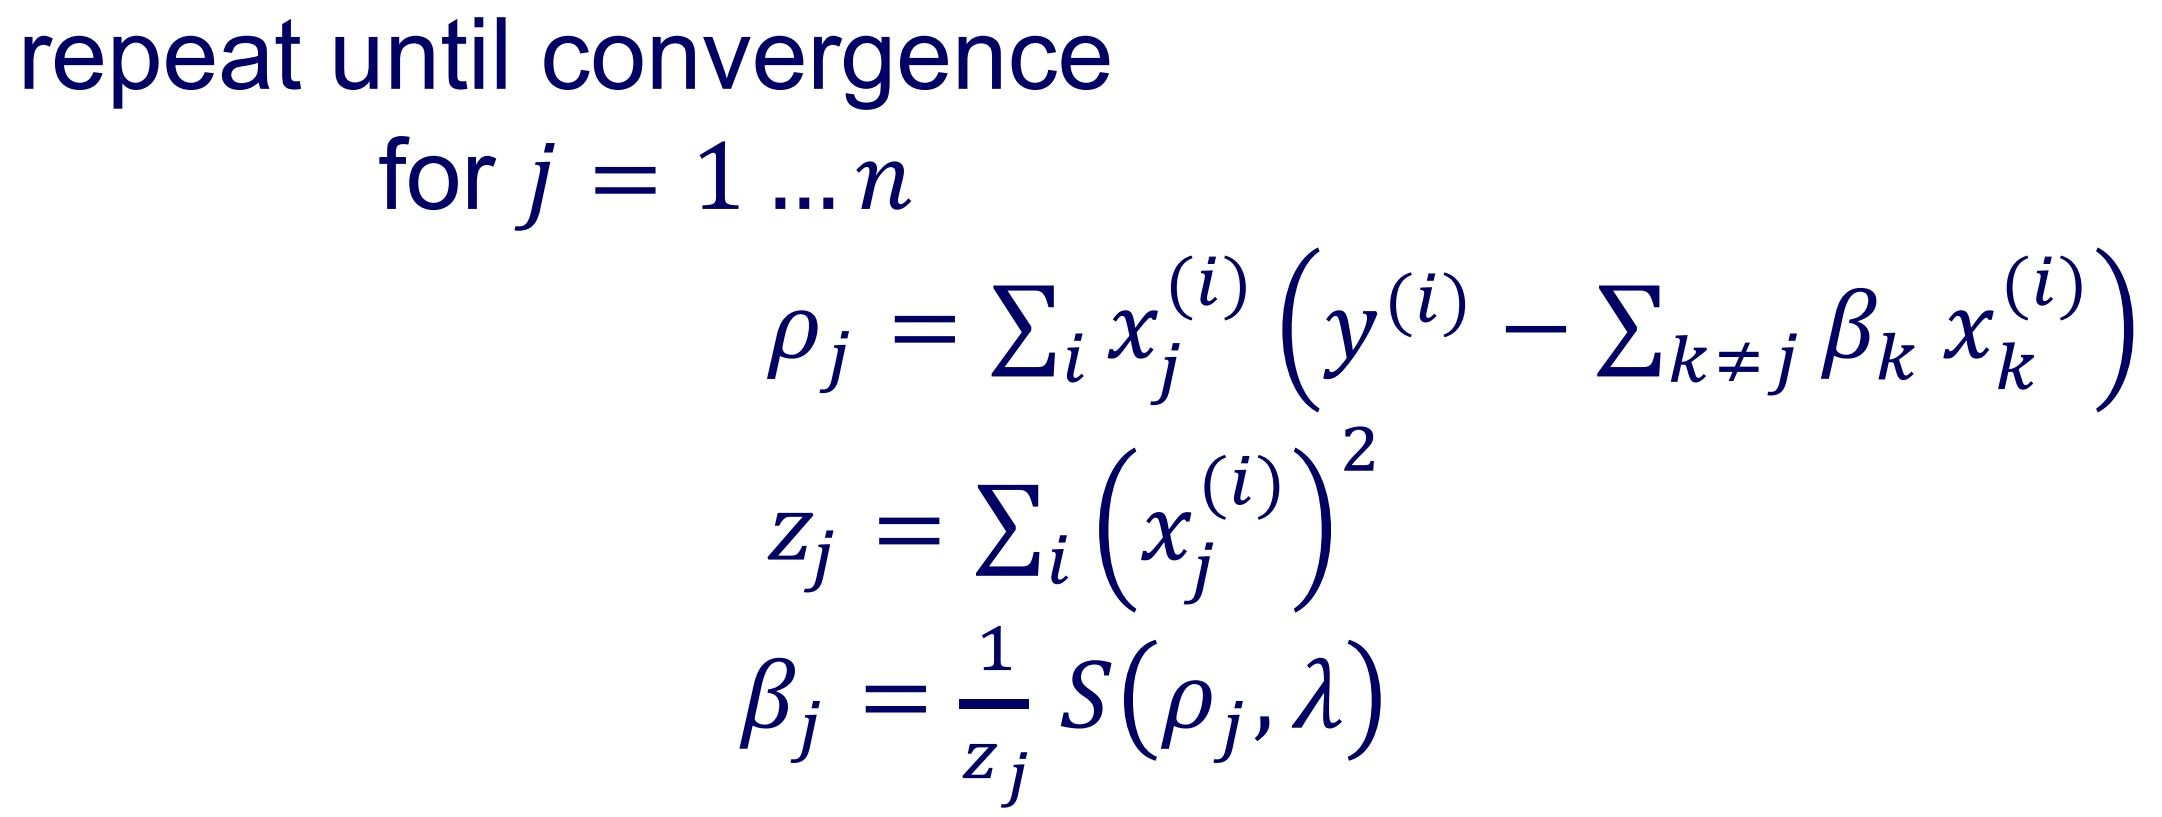
\includegraphics[width=0.6\linewidth]{snips/21_lasso-coordinate-descent-2.jpg}
    \begin{equation*}
        S(\rho, \lambda) =
        \begin{cases}
            \rho - \lambda &\text{if } \rho > \lambda \\ 
            0 &\text{if } -\lambda \leq \rho \leq \lambda \\ 
            \rho + \lambda &\text{if } \rho < -\lambda \\ 
        \end{cases}
    \end{equation*}

    \section{Ensembles}

    Bagging

    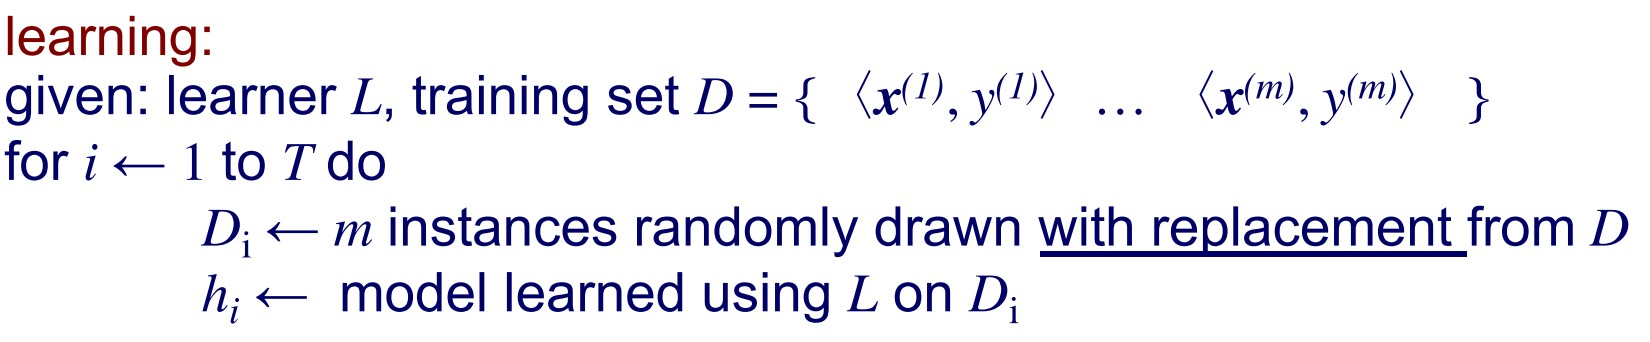
\includegraphics[width=0.8\linewidth]{snips/22_bagging.jpg}

    AdaBoost

    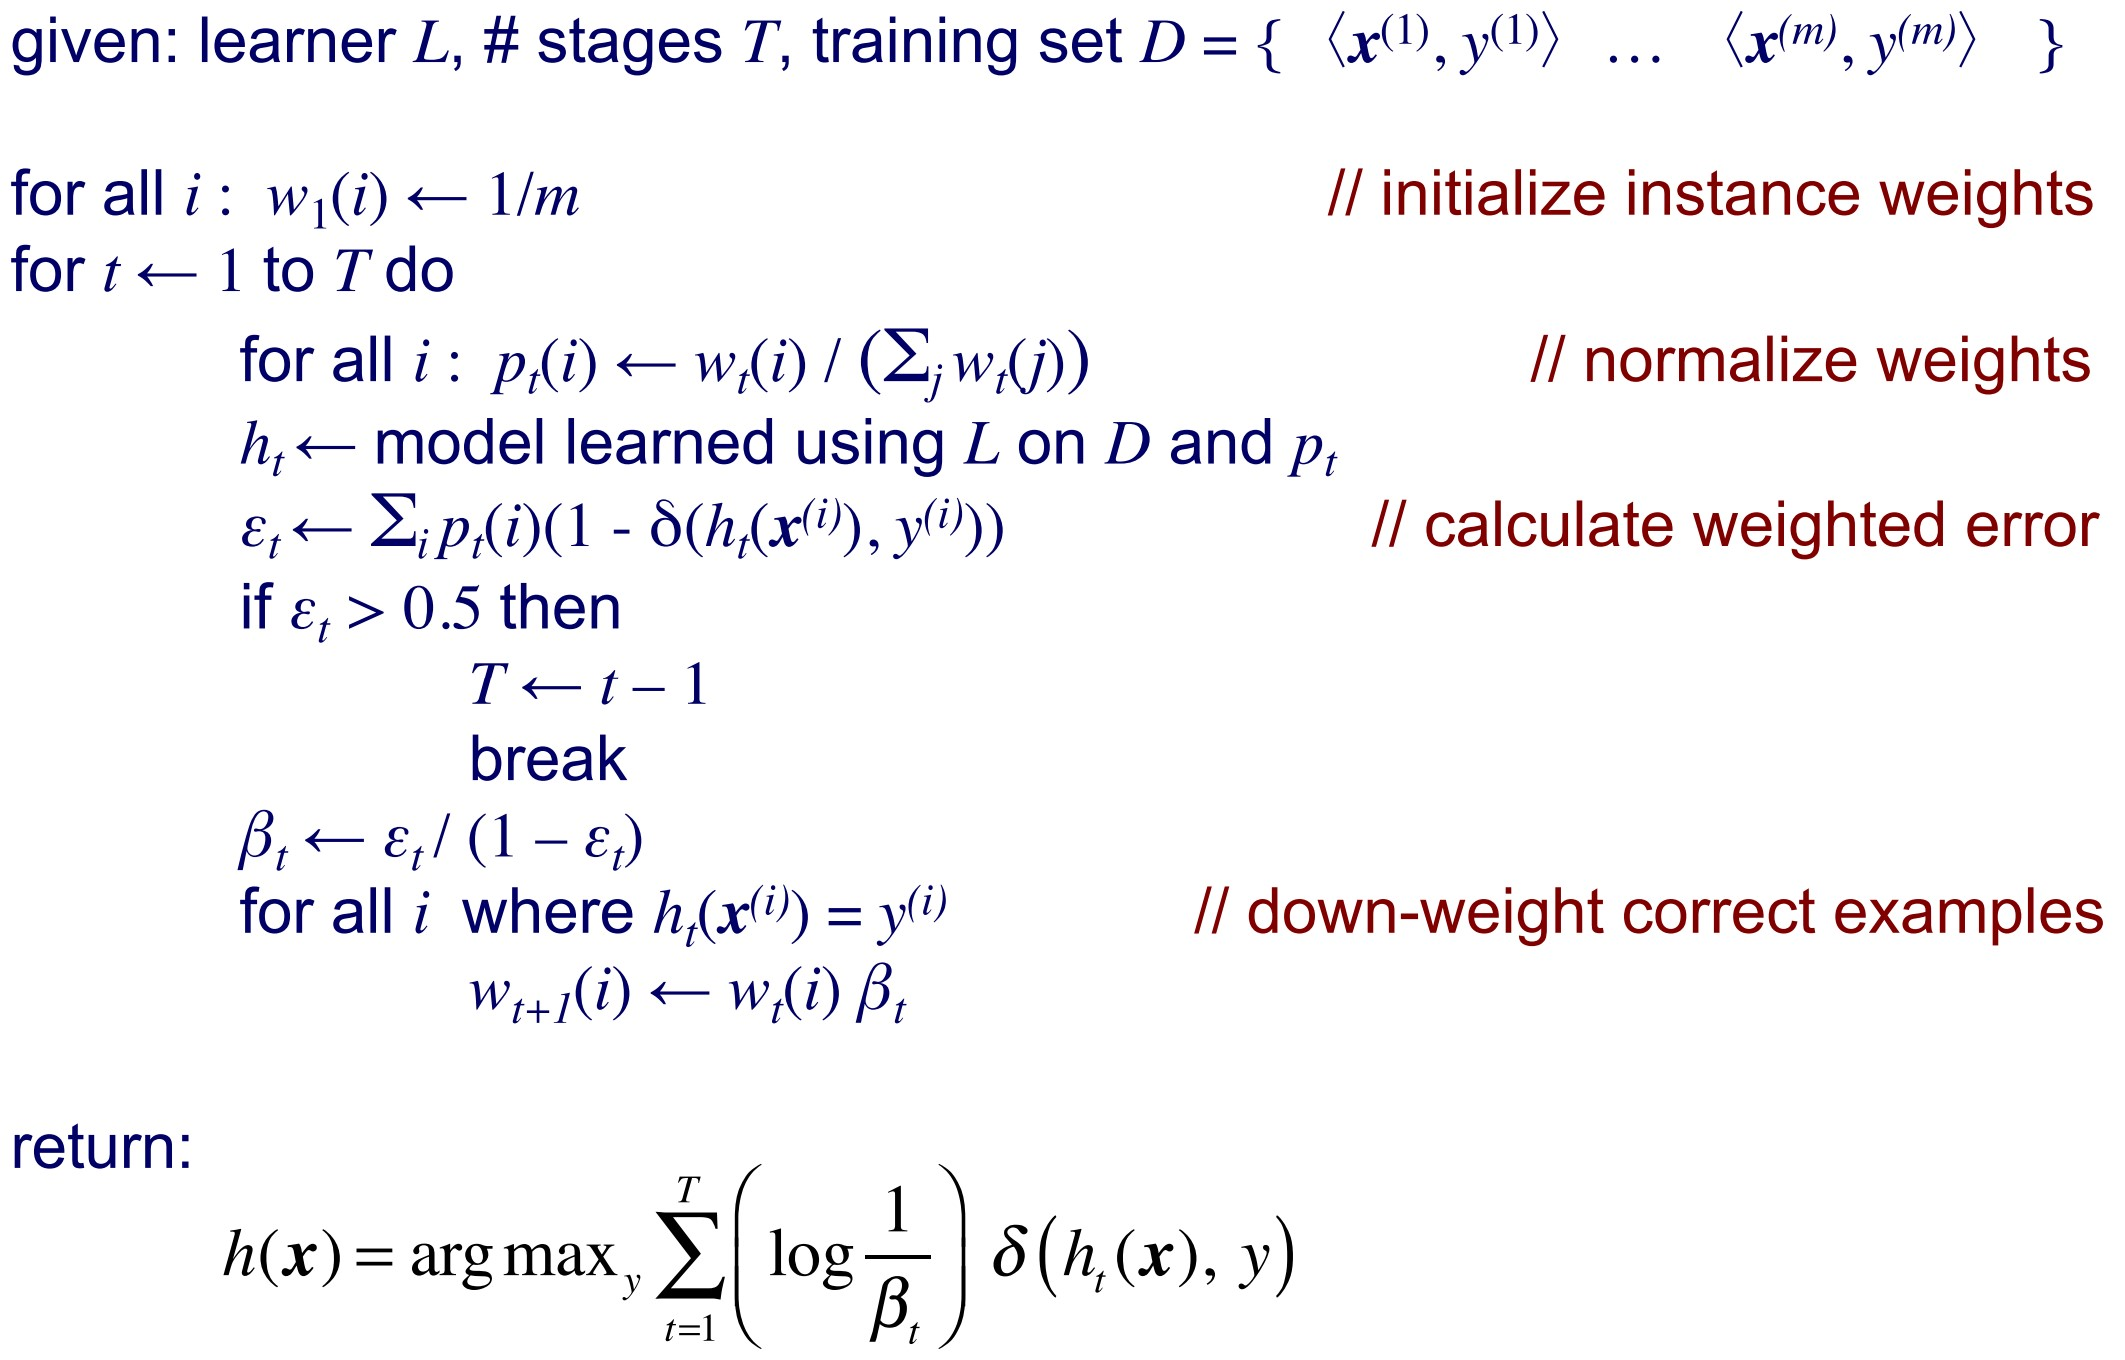
\includegraphics[width=0.9\linewidth]{snips/23_adaboost.jpg}

    Random Forest

    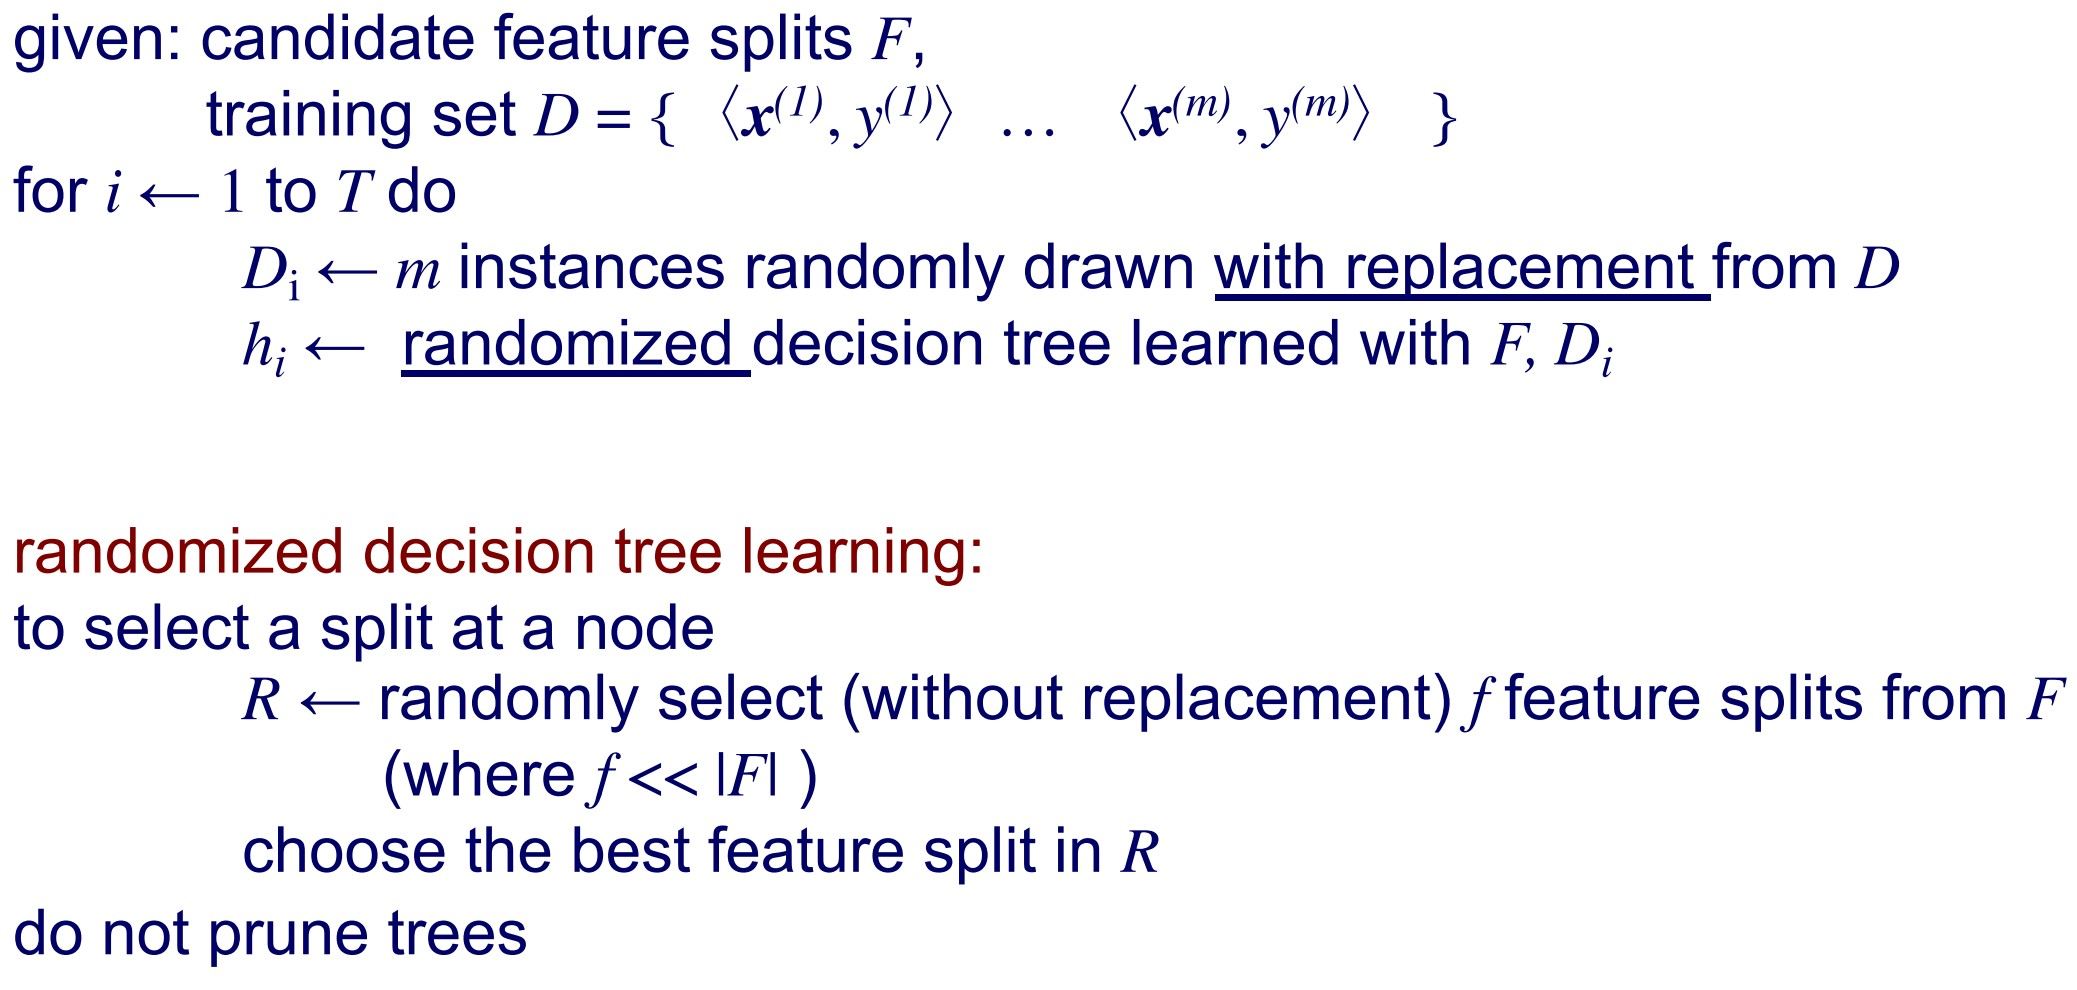
\includegraphics[width=0.9\linewidth]{snips/24_random-forest.jpg}   
    
    
    \section{Support Vector Machines}
    
    \begin{equation*}
    h(x) = \begin{cases} +1 \quad \text{if } \bold{w}^T \bold{x} + b > 0 \\ -1 \quad \text{o/w} \end{cases}
    \end{equation*}
    \begin{equation*}
        \text{margin}_D (h) = \frac{1}{2} \bold{\hat{w}}^T (x_+ - x_-) = \frac{1}{||\bold{w}||_2}
    \end{equation*}
    \begin{align*}
        \min_{\bold{w},b}& \frac{1}{2} || \bold{w}||_2^2
        \qquad \text{(hard-margin)}
        \\
        \text{ s.t. }& y^{(i)} (\bold{w}^T \bold{x}^{(i)} + b) \geq 1 \; \forall i
        \\
        \min_{\bold{w},b,\xi^{(i)}}& \frac{1}{2} || \bold{w}||_2^2 + C \sum_{i=1}^m \xi^{(i)}
        \qquad \text{(soft-margin)}
        \\
        \text{ s.t. }& y^{(i)} (\bold{w}^T \bold{x}^{(i)} + b) \geq 1-\xi^{(i)}, \; \xi^{(i)} \geq 0 \; \forall i
        \\
        \max_{\alpha_1,\dots, \alpha_m}& \sum_{i=1}^m \alpha_i - \frac{1}{2} \sum_{j=1}^m \sum_{i=1}^m \alpha_j \alpha_k y^{(j)} y^{(k)} \left(\bold{x}^{(j)} \cdot \bold{x}^{(k)} \right)
        \\
        \text{ s.t. }& \alpha_i \geq 0,\; \sum_{i=1}^m \alpha_i y^{(i)} = 0
        \qquad \text{(h-m dual)}
    \end{align*}
    \begin{align*}
        k(x,z) &= (x \cdot z)^d
        & \text{(polynomial d)}
        \\
        k(x,z) &= (x \cdot z + 1)^d
        & \text{(polynomial up-to d)}
        \\
        k(x,z) &= \exp \left( -\gamma ||x-z||^2 \right)        
        & \text{(RBF)}
    \end{align*}    
    
    \section{Learning Theory}
    
    \begin{equation*}
        error_{D}(h) = P_{x \in D} \left( c(x) \neq h(x)\right)
    \end{equation*}
    \begin{equation*}
        error(h) \leq error_D(h) + \sqrt{\frac{VC (\log(2m/VC) + 1) + \log(4/\delta)}{m}}
    \end{equation*}
    
    \begin{align*}
        m &\geq \frac{1}{\varepsilon} \left( \ln |H| + \ln \left(\frac{1}{\delta} \right) \right)
        \;\;(\textrm{finite H)}
        \\
        m &\geq \frac{1}{\varepsilon} \left( 4 \log_2 \left(\frac{2}{\delta} \right) + 8 \text{VC-dim}(H) \log_2 \left(\frac{13}{\varepsilon} \right) \right)
        %\;\; (|H| = \textrm{finite} or \infty)
        \\
        m &\geq \frac{1}{\varepsilon^2} \left( \ln |H| + \ln \left(\frac{1}{\delta} \right) \right)
        \;\;\text{(agnostic learning)}
    \end{align*}
    
    \begin{align*}
        m < \max \left( \frac{1}{\varepsilon} \log \left(\frac{1}{\delta}\right), \frac{\text{VC-dim}(C) -1}{32\varepsilon}\right) \\
        \implies \text{w.p. } \delta, \; error_D(h) > \varepsilon
    \end{align*}
    \begin{equation*}
        VC \leq \frac{4R^2}{\text{margin}_D(h)^2}
    \end{equation*}
    
    {
        \centering
        Halving algorithm
        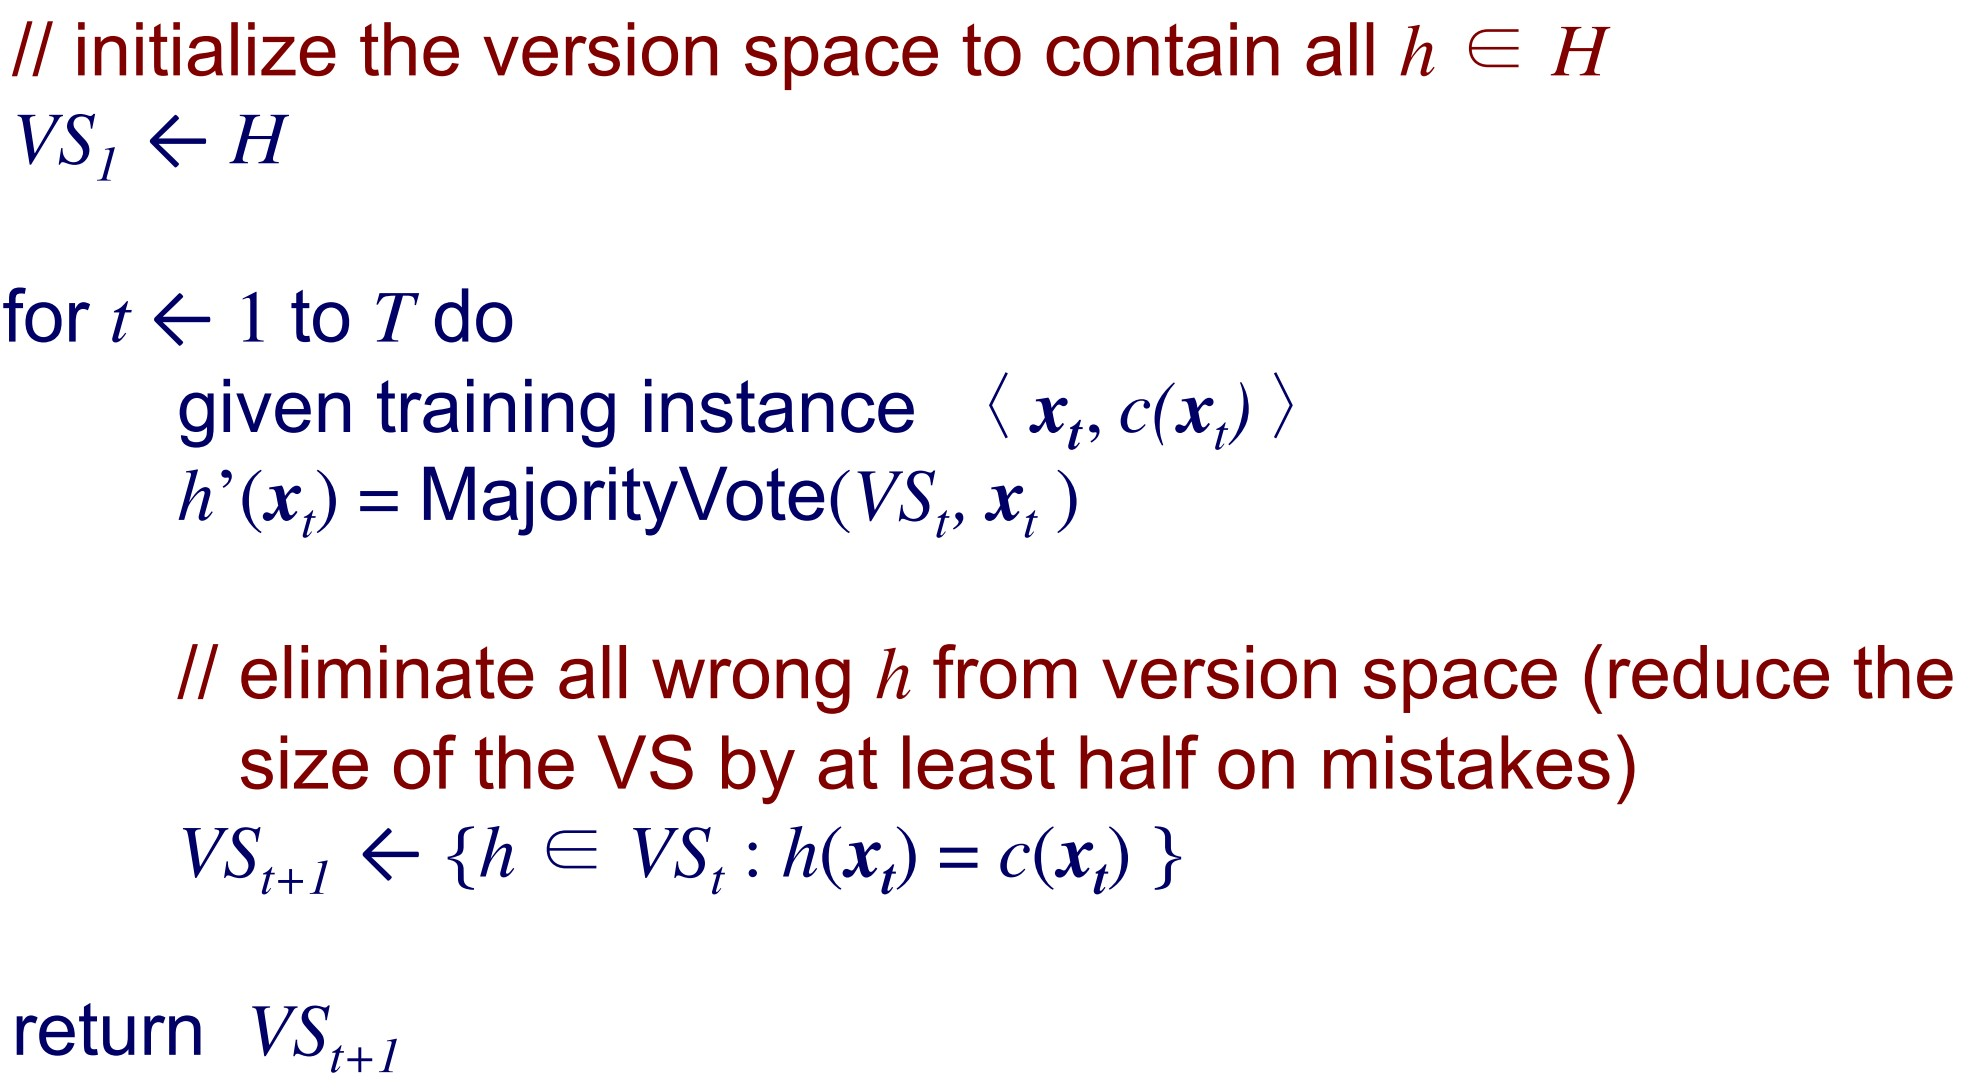
\includegraphics[width=0.8\linewidth]{snips/28_halving-algorithm.jpg}
    
        Weighted majority
        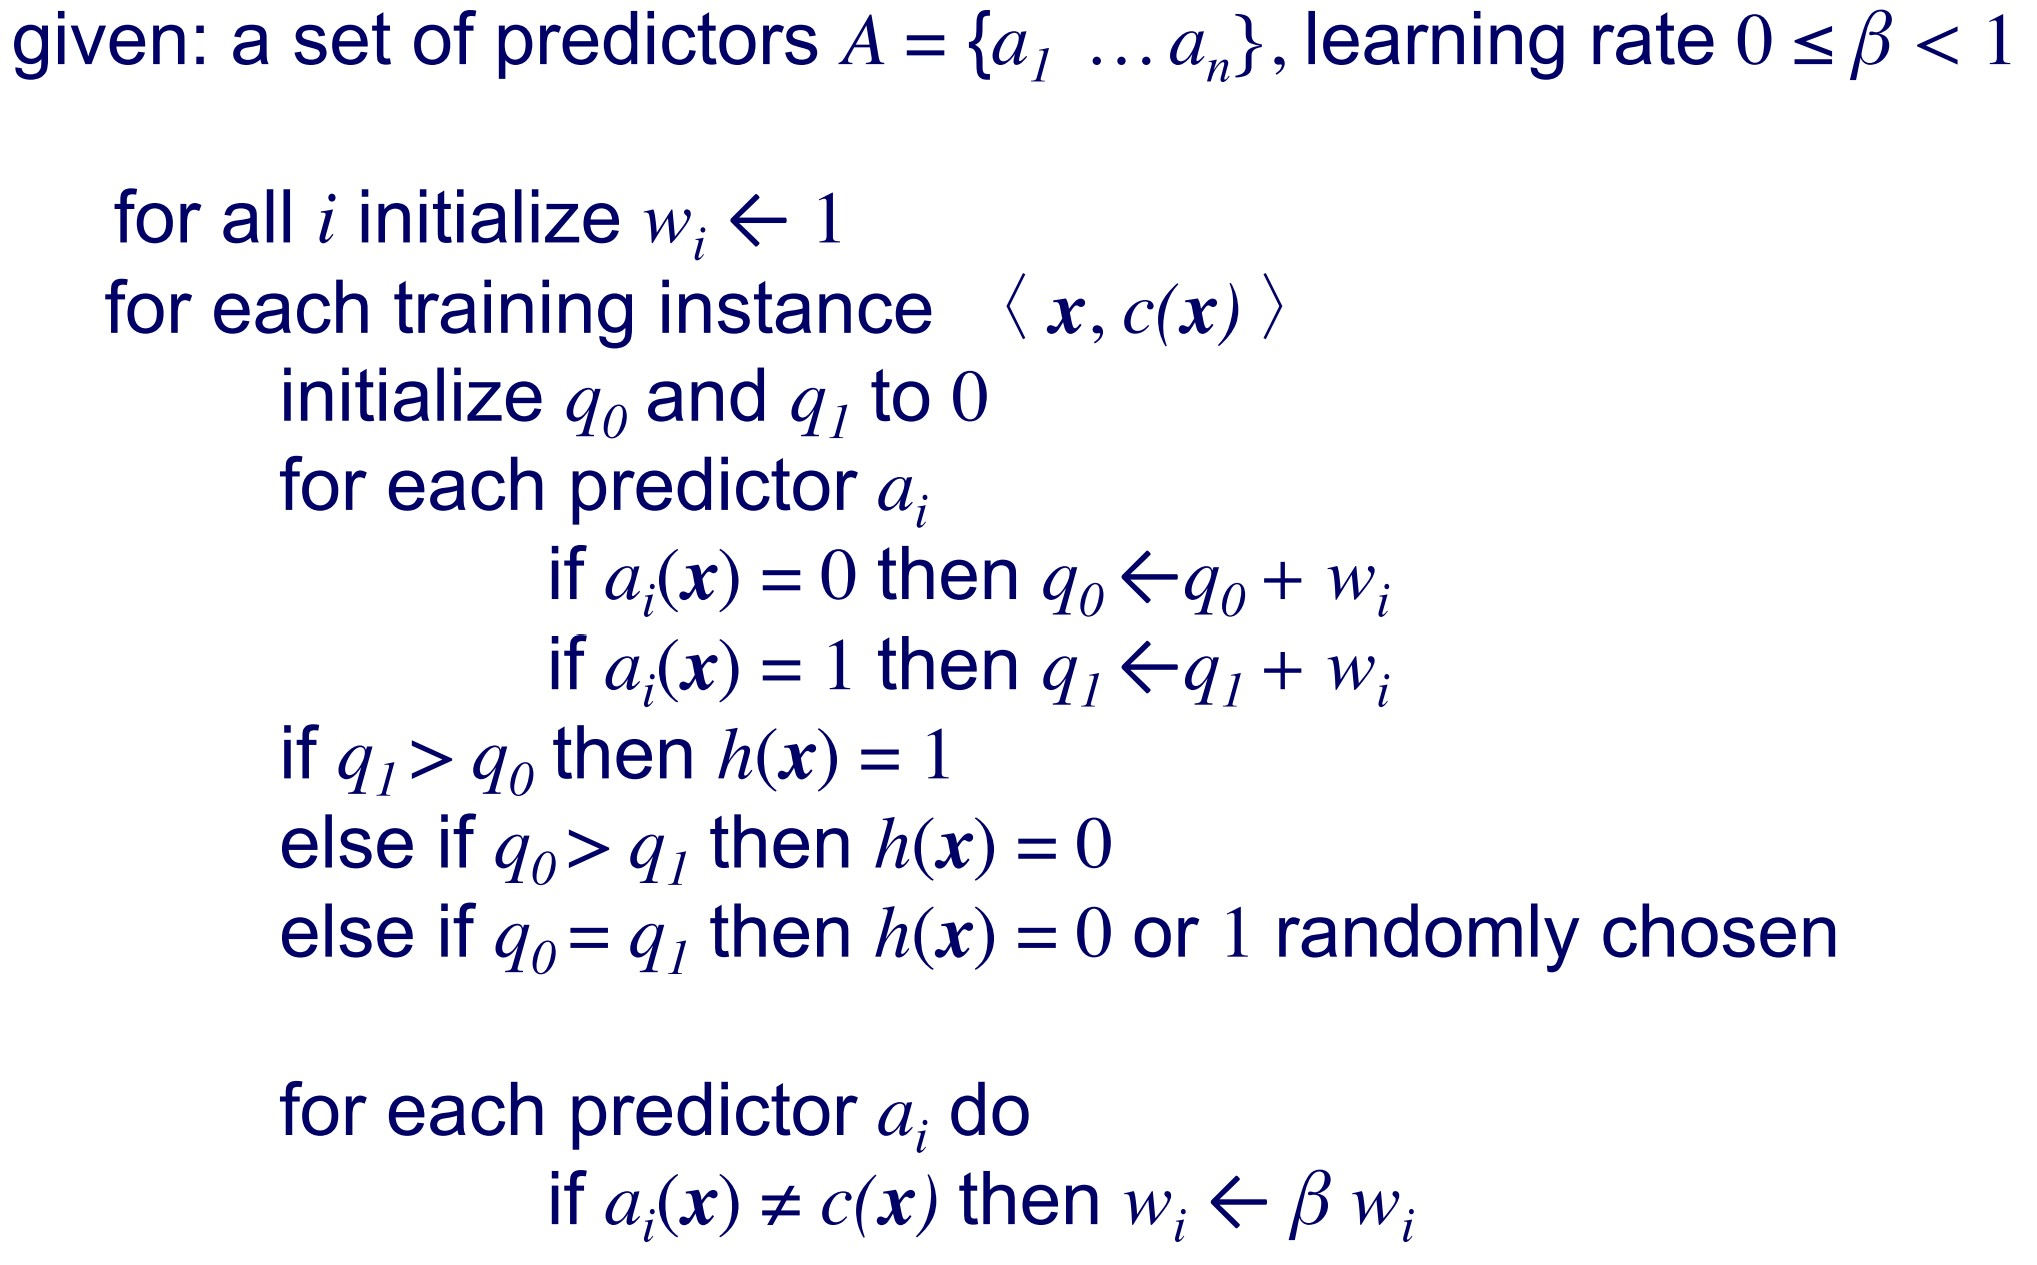
\includegraphics[width=0.8\linewidth]{snips/29_weighted-majority.jpg}
        
    }
    
    
    
    \section{Bias, Variance, \& Overfitting}
    
    \begin{align*}
        E_D \left[ \left( f(x;D) - E[y|x]\right)^2 \right] = \left( E_d[f(x;D)] - E[y|x]\right)^2 \\
        + E_D \left[ (f(x;D) - E_D[f(x;D)])^2\right]
    \end{align*}
    \begin{align*}
        E \left[  \left(y-f(x; D)\right)^2 \right] = E \left[  \left(y-E[y|x]\right)^2 \mid x,D \right] \\
        + \left( f(x;D) - E[y|x]\right)^2
    \end{align*}
    % \begin{align*}
    %     \text{Bias}[\hat{\theta}] = E[\hat{\theta}] - \theta
    % \end{align*}
    \begin{align*}
        h \in H \text{ overfits if } \exists h' \in H         \text{ s.t. } error(h) > error(h')  \\
        \text{ and } error_D(h) < error_D(h')
    \end{align*}
    
    % \subsection{xCode}
    % Subsetction text
    
    
    \section{Reinforcement Learning}
    
    \begin{equation*}
        V^{\pi} (s) = \sum_{t=0}^\infty \gamma^t E[r_t]
    \end{equation*}
    \begin{equation*}
        \pi^* = \arg \max_\pi V^\pi (s) \quad \forall s
    \end{equation*}
    \begin{equation*}
        Q(s,a) = E[r(s,a)] + \gamma E_{s'|s,a} [V^*(s')]
    \end{equation*}
    \begin{equation*}
        \pi^* (s) = \arg \max_a Q(s,a)
    \end{equation*}
    \begin{equation*}
        P(a_i|s) = \frac{c^{\hat{Q}(s,a_i)}}{\sum_j c^{\hat{Q}(s,a_j)}}
    \end{equation*}
    
    Q Learning (Deterministic)
    
    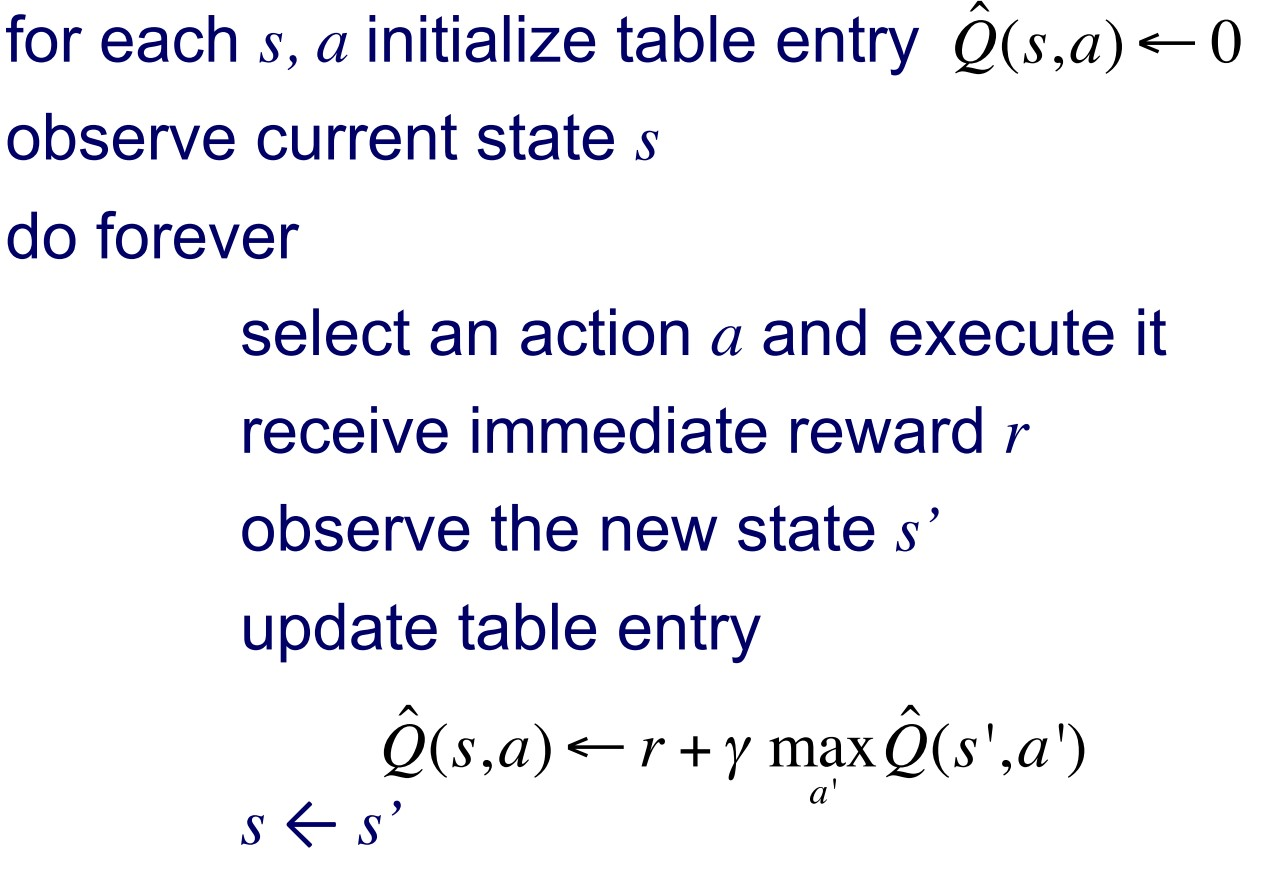
\includegraphics[width=0.65\linewidth]{snips/31_q-learning.jpg}

    Q Learning (Non-deterministic)
    
    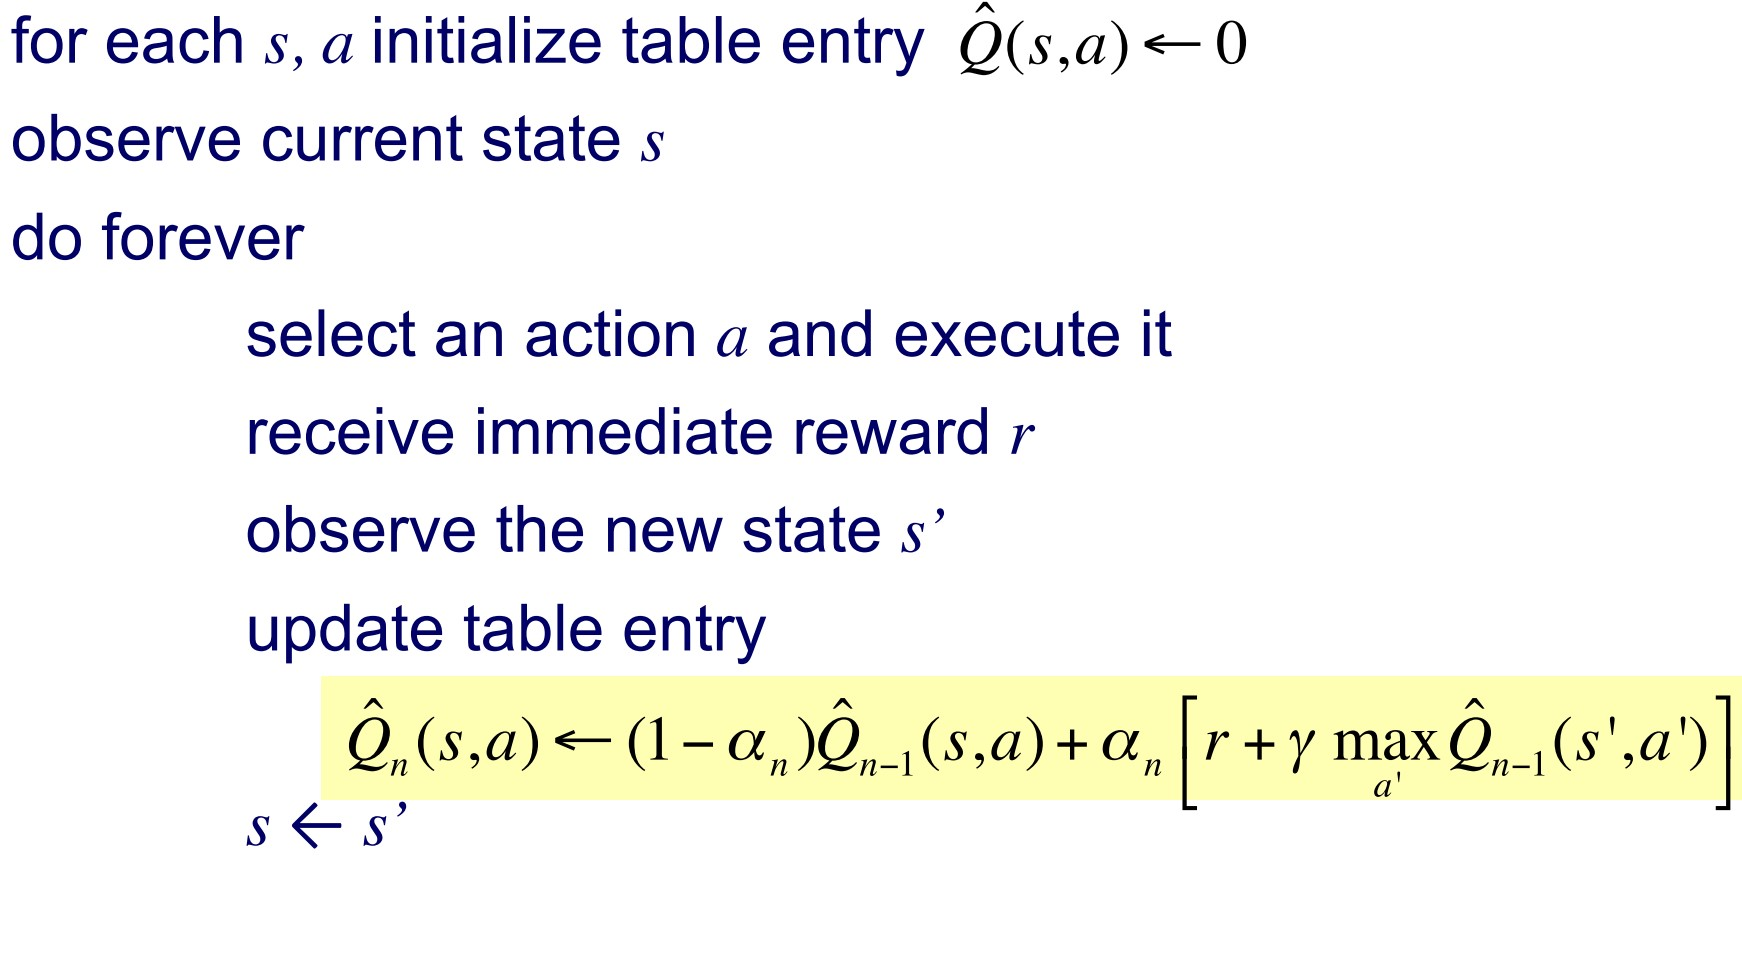
\includegraphics[width=0.85\linewidth]{snips/32_q-learning-non-deterministic.jpg}

    AlphaZero
    
    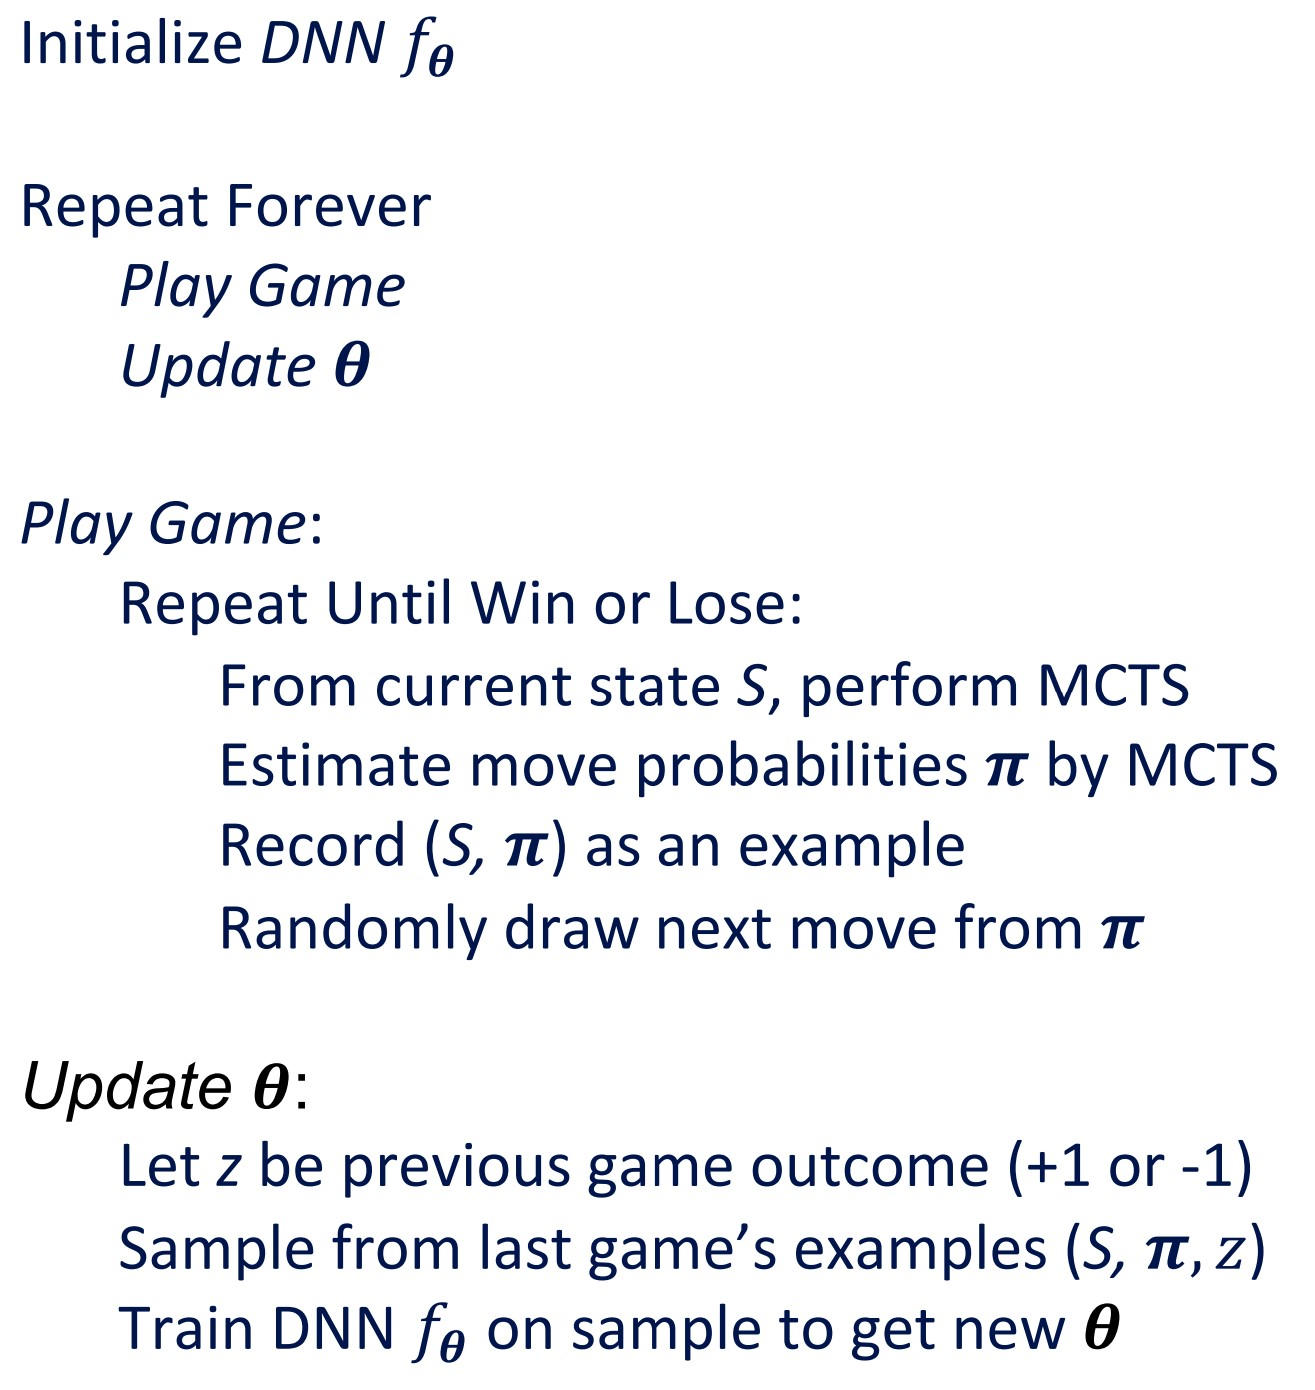
\includegraphics[width=0.7\linewidth]{snips/33_alpha-zero.jpg}
    
    % You can even have references
    % \rule{0.3\linewidth}{0.25pt}
    % \scriptsize
    % \bibliographystyle{abstract}
    % \bibliography{refFile}
\end{multicols}
\end{document}